\documentclass[10pt,a4paper,openany]{book}
% Векторные русских шрифтов в PDF
% Необходимо установить также пакеты cm-super и cm-unicode
\usepackage{cmap}
\usepackage[X2, T2A]{fontenc}
\usepackage[utf8]{inputenc}
\usepackage[english,french,german,italian,russian]{babel}
\usepackage{indentfirst}                % Красная строка в первом абзаце
% Подключение amsmath также даёт поддержку автоматических \dots
% см. http://tex.stackexchange.com/questions/77737/dots-versus-ldots-is-there-a-difference
% см. http://tex.stackexchange.com/questions/117730/what-is-the-difference-between-ldots-and-cdots
\usepackage{amsmath} % разрешить \texttt и аналогичные в формулах
\usepackage{amssymb} % дополнительные математические символы
\usepackage{graphicx} % поддержка изображений

%\usepackage{amsfonts, eucal, bm, color, }

\usepackage{algorithm, algorithmic}     % 'algorithm' environments
\floatname{algorithm}{Алгоритм}

\usepackage{array}                      % Новые команды для работы с таблицами, см. также ниже доопределение стилей ячеек L, C, R
\usepackage{arydshln}                   % dash lines in tables
\usepackage{caption}                    % titles for figures
\usepackage{csquotes}
\usepackage{enumerate}
\usepackage{enumitem}                   % кастомизация itemize/enumerate, напр. отказ от indent
\usepackage{fancybox}                   % страница в рамке
\usepackage{float}			% sub figures
\usepackage[totoc=true]{idxlayout}      % балансировка индексов на последней странице, индекс в ToC
\usepackage{lscape}                     % поддержка поворота страниц на 90 градусов для широких таблиц
\usepackage{multicol}                   % поддержка колонок
\setlength{\columnsep}{0.1cm}
\usepackage{multirow}                   % multirow cells in tables
%\usepackage{subfig}			% sub figures
\usepackage{subcaption}         % sub figures, incompatible with package{subfig}
\usepackage{tikz}                       % векторная графика внутри TeX
\usepackage{tablefootnote}		% footnote в таблицах
\usepackage{wrapfig}			% sub figures
\usepackage{textcomp}                   % \No support
\usepackage{cjhebrew}
\usepackage{import}

\usepackage[left=1.84cm, right=1.5cm, paperwidth=14cm, top=1.8cm, bottom=2cm, height=19.8cm, paperheight=20cm]{geometry}

% Необходимо установить biblatex-gost
% и переключить сборку библиографии на biber
\usepackage[parentracker=true,
  backend=biber,
  hyperref=auto,
  language=auto,
  autolang=other,
  citestyle=gost-numeric,
  defernumbers=true,
  bibstyle=gost-numeric,
  sortlocale=ru_RU
]{biblatex}								% библиография по ГОСТу

\newcommand{\indexchapter}[1]{%
\chapter*{#1}%
\addcontentsline{toc}{chapter}{#1}%
}
\usepackage[xindy]{imakeidx}
\makeindex[program=texindy, options=-M mystyle.xdy -L russian -C utf8]
\indexsetup{level=\indexchapter,toclevel=chapter}

\let\oldindex\index

\makeatletter
\renewcommand{\index}[2][\imki@jobname]{%
	\oldindex[#1]{\detokenize{#2}}%
}
\makeatother

% поддержка гиперссылок; гиперссылки в pdf, должен быть последним загруженным пакетом
\ifx\pdfoutput\undefined
    \usepackage[unicode,dvips]{hyperref}
\else
    \usepackage[pdftex,colorlinks,unicode,bookmarks]{hyperref}
\fi

%\paperwidth=16.8cm \oddsidemargin=0cm \evensidemargin=0cm \hoffset=-0.33cm \textwidth=13.2cm
%\paperheight=24cm \voffset=-0.4cm \topmargin=0cm \headsep=0cm \headheight=0cm \textheight=19.8cm \footskip=0.9cm

% параметры PDF файла
\hypersetup{
    pdftitle={Защита информации},
    pdfauthor={Э. М. Габидулин, А. С. Кшевецкий, А. И. Колыбельников, С. М. Владимиров},
    pdfsubject=учебное пособие,
    pdfkeywords={защита информации, криптография, МФТИ}
}

% добавить точку после номера секции, раздела и~т.\,д.
\makeatletter
\def\@seccntformat#1{\csname the#1\endcsname.\quad}
\def\numberline#1{\hb@xt@\@tempdima{#1\if&#1&\else.\fi\hfil}}
\makeatother

% перенос слов с тире
%\lccode`\-=`\-
%\defaulthyphenchar=127

% изменить подписи к рисункам, таблицам и~т.\,д.
\captionsetup{labelsep=endash}          % Нумерационный заголовок и текст разделяются тире
\captionsetup{textformat=simple}        % Текст подписи будет напечатан как есть
%\captionsetup[table]{position=above}    % вертикальные отступы подписи таблицы для случая, когда подпись вверху
%\captionsetup[figure]{position=below}   % вертикальные отступы подписи рисунка для случая, когда подпись внизу

%% стиль главы и секции вверху страницы
%\pagestyle{fancy}
%%\renewcommand{\chaptermark}[1]{\markboth{#1}{}}
%\renewcommand{\sectionmark}[1]{\markright{#1}{}}
%
%%\fancyhf{}
%%\fancyfoot[СE,CO]{\thepage}
%%\fancyhead[LE]{\textsc{\nouppercase{\leftmark}}}
%\fancyhead[RO]{\textsc{\nouppercase{\rightmark}}}
%
%\fancypagestyle{plain}{ %
%\fancyhf{}                              % remove everything
%\renewcommand{\headrulewidth}{0pt}      % remove lines as well
%\renewcommand{\footrulewidth}{0pt}}

% запретить выходить за границы страницы
\sloppy

\newtheorem{theorem}{Теорема}[section]
\newtheorem{lemma}[theorem]{Лемма}
\newtheorem{definition}[theorem]{Определение}
\newtheorem{property}[theorem]{Утверждение}
\newtheorem{corollary}[theorem]{Следствие}
%\newtheorem{algorithm}[theorem]{Алгоритм}
\newtheorem{remark}[theorem]{Замечание}
\newcommand{\proof}{\noindent\textsc{Доказательство.\ }}

%\newtheorem{example}{\textsc{\textbf{Пример}}}
\newcommand{\example}{\textsc{\textbf{Пример.}} }
\newcommand{\exampleend}

\DeclareMathOperator{\ord}{ord}
\newcommand{\set}[1]{\mathbb{#1}}
\newcommand{\group}[1]{\mathbb{#1}}
\newcommand{\E}{\group{E}}
\newcommand{\F}{\group{F}}
\newcommand{\GF}[1]{\group{GF}(#1)}
\newcommand{\Gr}{\group{G}}
\newcommand{\Mod}{\operatorname{mod}}
\newcommand{\R}{\group{R}}
\newcommand{\Z}{\group{Z}}
\newcommand{\MAC}{\textrm{MAC}}
\newcommand{\HMAC}{\textrm{HMAC}}
\newcommand{\PK}{\textrm{PK}}
\newcommand{\SK}{\textrm{SK}}

\newcommand{\langde}[1]{нем. \foreignlanguage{german}{\textit{#1}}}
\newcommand{\langfr}[1]{фр. \foreignlanguage{french}{\textit{#1}}}
\newcommand{\langen}[1]{англ. \foreignlanguage{english}{\textit{#1}}}
\newcommand{\langit}[1]{итал. \foreignlanguage{italian}{\textit{#1}}}
\newcommand{\langlat}[1]{лат. \foreignlanguage{italian}{\textit{#1}}}

% Русская типографика
\renewcommand\leq{\leqslant}
\renewcommand\geq{\geqslant}
\renewcommand\emptyset{\varnothing}
\renewcommand\kappa{\varkappa}
\renewcommand\epsilon{\varepsilon}
\renewcommand\phi{\varphi}
\renewcommand*{\No}{\textnumero}

% Для раздела с задачами
\newcommand{\taskinit}{\newcounter{task-section}\setcounter{task-section}{0}\newcounter{task-number}}
\newcommand{\tasksection}{\addtocounter{task-section}{1}\setcounter{task-number}{0}}
\newcommand{\tasknumber}{\textbf{\No\addtocounter{task-number}{1}\arabic{task-section}.\arabic{task-number}.}~~}

%Наконец, существует способ дублировать знаки операций, который мы приведём безо всяких пояснений. Включив
%\newcommand*{\hm}[1]{#1\nobreak\discretionary{}{\hbox{\mathsurround=0pt #1}}{}}
%в преамбулу, можно написать $a\hm+b\hm+c\hm+d$, при этом в формуле a\hm+b\hm+c\hm+d при переносе знак + будет продублирован.

% Дублирование символов бинарных операций ("+", "-", "="), набранных в строчных формулах, при переносе на другую строку:
%%begin{latexonly}
%\renewcommand\ne{\mathchar"3236\mathchar"303D\nobreak
%      \discretionary{}{\usefont
%      {OMS}{cmsy}{m}{n}\char"36\usefont
%      {OT1}{cmr}{m}{n}\char"3D}{}}
%\begingroup
%\catcode`\+\active\gdef+{\mathchar8235\nobreak\discretionary{}%
% {\usefont{OT1}{cmr}{m}{n}\char43}{}}
%\catcode`\-\active\gdef-{\mathchar8704\nobreak\discretionary{}%
% {\usefont{OMS}{cmsy}{m}{n}\char0}{}}
%\catcode`\=\active\gdef={\mathchar12349\nobreak\discretionary{}%
% {\usefont{OT1}{cmr}{m}{n}\char61}{}}
%\endgroup
%\def\cdot{\mathchar8705\nobreak\discretionary{}%
% {\usefont{OMS}{cmsy}{m}{n}\char1}{}}
%\def\times{\mathchar8706\nobreak\discretionary{}%
% {\usefont{OMS}{cmsy}{m}{n}\char2}{}}
%\mathcode`\==32768
%\mathcode`\+=32768
%\mathcode`\-=32768
%%end{latexonly}

% Упрощение создания таблиц с длинным текстом в ячейках
\newcolumntype{L}[1]{>{\raggedright\let\newline\\\arraybackslash\hspace{0pt}}m{#1}}
\newcolumntype{C}[1]{>{\centering\let\newline\\\arraybackslash\hspace{0pt}}m{#1}}
\newcolumntype{R}[1]{>{\raggedleft\let\newline\\\arraybackslash\hspace{0pt}}m{#1}} 

% Рекомендация для latex'а не разрывать inline-формулы
\binoppenalty=9999
\relpenalty=9999


\addbibresource{bibliography.bib}
\begin{document}
\selectlanguage{russian}

\title{Защита информации \\ Учебное пособие}
\author{Габидулин Эрнст Мухамедович \\ Кшевецкий Александр Сергеевич \\ Колыбельников Александр Иванович \\ Владимиров Сергей Михайлович}
\date{
 %   \textbf{\textsc{Черновой вариант. Может содержать ошибки.}} \\
%    \today
}
\maketitle
\setcounter{page}{3}

\newpage
%\thispagestyle{empty}
\setcounter{tocdepth}{2}
\tableofcontents
%\thispagestyle{empty}
\newpage

%\lhead[\leftmark]{}
%\rhead[]{\rightmark}

\chapter*{Предисловие}
\addcontentsline{toc}{chapter}{Предисловие}
\markboth{ПРЕДИСЛОВИЕ}{ПРЕДИСЛОВИЕ}
\selectlanguage{russian}

В настоящем пособии рассмотрены только основные математические методы защиты информации, и среди них главный акцент сделан на криптографическую защиту, которая включает симметричные и несимметричные методы шифрования, формирование секретных ключей, протоколы ограничения доступа и аутентификации сообщений и пользователей. Кроме того, в пособии рассматриваются типовые уязвимости операционных и информационно-вычислительных систем.

\section*{Благодарности}
\addcontentsline{toc}{section}{Благодарности}
Авторы пособия благодарят студентов, аспирантов и сотрудников Московского физико-технического института (государственного университета), которые помогли с подготовкой, редактированием и поиском ошибок в тексте.

\setlength{\columnsep}{0.5em}
\begin{multicols}{2}
\begin{small}
\begin{itemize}[leftmargin=0.5em]\itemsep1pt \parskip0pt \parsep0pt

	\item[] Владимир Аверьянов\begin{tiny} (201-113 гр.)\end{tiny} %rfoofr
	\item[] Руслан Агишев\begin{tiny} (201-314 гр.)\end{tiny} %agruslan

	\item[] Алипаша Бабаев\begin{tiny} (201-311 гр.)\end{tiny} %alishnik
	\item[] Олег Бабин\begin{tiny} (201-415 гр.)\end{tiny} %olegrok
	\item[] Татьяна Бакланова\begin{tiny} (201-211 гр.)\end{tiny}
	\item[] Дмитрий Банков\begin{tiny} (201-011 гр.)\end{tiny}
	\item[] Александр Белов\begin{tiny} (201-214 гр.)\end{tiny}
	\item[] Даниил Бершацкий\begin{tiny} (201-012 гр.)\end{tiny}
	\item[] Анастасия Бодрова\begin{tiny} (201-218 гр.)\end{tiny} %AnastasiaBodrova
	\item[] Дмитрий Бородий\begin{tiny} (201-112 гр.)\end{tiny}
	\item[] Евгений Брицын\begin{tiny} (201-312 гр.)\end{tiny} %ebritsyn
	\item[] Олег Бусловский\begin{tiny} (201-219 гр.)\end{tiny} %oledzzka

	\item[] Вадим Варнавский\begin{tiny} (201-213 гр.)\end{tiny}
	\item[] Илья Васильев\begin{tiny} (201-217 гр.)\end{tiny}
	\item[] Эмиль Вахитов\begin{tiny} (201-114 гр.)\end{tiny}
	\item[] Дмитрий Вербицкий\begin{tiny} (201-119 гр.)\end{tiny}
	\item[] Константин Виноградов\begin{tiny} (201-114 гр.)\end{tiny} %Vikont133

	\item[] Тагир Гадельшин\begin{tiny} (201-119 гр.)\end{tiny}
	\item[] Марат Гаджибутаев\begin{tiny} (201-018 гр.)\end{tiny}
	\item[] Тимур Газизов\begin{tiny} (201-317 гр.)\end{tiny} %RiderOnTheStorm
	\item[] Ильназ Гараев\begin{tiny} (201-113 гр.)\end{tiny}
	\item[] Евгений Глушков\begin{tiny} (201-012 гр.)\end{tiny}
	\item[] Иван Голованов\begin{tiny} (201-312 гр.)\end{tiny} %ivangolovanov; legendawes, legendawes1
	\item[] Андрей Горбунов\begin{tiny} (201-116 гр.)\end{tiny} %goriand
	\item[] Елена Гундрова\begin{tiny} (201-214 гр.)\end{tiny}
	\item[] Алексей Гусаров\begin{tiny} (201-216 гр.)\end{tiny}
	\item[] Наталья Гусева\begin{tiny} (201-216 гр.)\end{tiny} %g-n-ev

	\item[] Андрей Диденко\begin{tiny} (201-311 гр.)\end{tiny} %DidenkoAndre
	\item[] Олег Дробот\begin{tiny} (201-317 гр.)\end{tiny} %tobord

	\item[] Дмитрий Ермилов\begin{tiny} (201-311 гр.)\end{tiny} %schnee-katze

	\item[] Сергей Жестков\begin{tiny} (201-013 гр.)\end{tiny}
	\item[] Андрей Житов\begin{tiny} (201-114 гр.)\end{tiny} %zhitHappens

	\item[] Виталий Занкин\begin{tiny} (201-111 гр.)\end{tiny} %zankin
	\item[] Дмитрий Зборовский\begin{tiny} (201-119 гр.)\end{tiny}

	\item[] Марат Ибрагимов\begin{tiny} (201-114 гр.)\end{tiny}
	\item[] Александр Иванов\begin{tiny} (201-011 гр.)\end{tiny}
	\item[] Александр Иванов\begin{tiny} (201-019 гр.)\end{tiny}
	\item[] Атнер Иванов\begin{tiny} (201-114 гр.)\end{tiny}
	\item[] Владимир Ивашкин\begin{tiny} (201-112 гр.)\end{tiny}

	\item[] Ирина Камалова\begin{tiny} (201-115 гр.)\end{tiny}
	\item[] Иван Киселёв\begin{tiny} (201-115 гр.)\end{tiny}
	\item[] Константин Ковальков\begin{tiny} (201-015 гр.)\end{tiny}
	\item[] Николай Козырский\begin{tiny} (201-417 гр.)\end{tiny} %NikolayKozyrskiy
	\item[] Федор Константинов\begin{tiny} (201-312 гр.)\end{tiny} %FRaKTT
	\item[] Анастасия Коробкина\begin{tiny} (201-312 гр.)\end{tiny} %korobkina
	\item[] Илья Копцов\begin{tiny} (201-115 гр.)\end{tiny} %IlyaKoptsov
	\item[] Андрей Кочетыгов\begin{tiny} (201-111 гр.)\end{tiny} %anko1774
	\item[] Сергей Кошечкин\begin{tiny} (201-213 гр.)\end{tiny}
	\item[] Александр Кравцов\begin{tiny} (201-116 гр.)\end{tiny}
	\item[] Анастасия Красавина\begin{tiny} (201-217 гр.)\end{tiny} %akrasavina
	\item[] Татьяна Красавина\begin{tiny} (201-214 гр.)\end{tiny} %tkrasav
	\item[] Виталий Крепак\begin{tiny} (201-013 гр.)\end{tiny}
	\item[] Егор Кривов\begin{tiny} (201-211 гр.)\end{tiny}
	\item[] Александр Кротов\begin{tiny} (201-011 гр.)\end{tiny}
	\item[] Ефим Крохин\begin{tiny} (201-217 гр.)\end{tiny} %Yefim-Krokhin
	\item[] Станислав Круглик\begin{tiny} (201-111 гр.)\end{tiny}
	\item[] Павел Крюков\begin{tiny} (200-916 гр.)\end{tiny} %pavelkryukov
	\item[] Аркадий Кудашов\begin{tiny} (201-317 гр.)\end{tiny} %ark85
	\item[] Денис Кудяков\begin{tiny} (201-314 гр.)\end{tiny} %Denis7775
	\item[] Егор Кузнецов\begin{tiny} (201-211 гр.)\end{tiny}
	\item[] Зулкаид Курбанов\begin{tiny} (201-113 гр.)\end{tiny}

	\item[] Всеволод Ливинский\begin{tiny} (201-216 гр.)\end{tiny} %Vsevolod-Livinskij
	\item[] Артемий Лузянин\begin{tiny} (201-312 гр.)\end{tiny} %artemluzyanin

	\item[] Егор Макарычев\begin{tiny} (201-115 гр.)\end{tiny}
	\item[] Иван Макеев\begin{tiny} (201-212 гр.)\end{tiny} %katala777
	\item[] Ольга Малюгина\begin{tiny} (201-111 гр.)\end{tiny}
	\item[] Алексей Мамаков\begin{tiny} (201-113 гр.)\end{tiny} %AlekseyMamakov
	\item[] Роман Маракулин\begin{tiny} (201-211 гр.)\end{tiny}
	\item[] Андрей Мартыненко\begin{tiny} (201-312 гр.)\end{tiny}
	\item[] Александр Матков\begin{tiny} (201-314 гр.)\end{tiny} %alexmatkov
	\item[] Артём Меринов\begin{tiny} (201-214 гр.)\end{tiny}
	\item[] Даниил Меркулов\begin{tiny} (201-111 гр.)\end{tiny}
	\item[] Олег Милосердов\begin{tiny} (201-016 гр.)\end{tiny}
	\item[] Дао Куанг Минь\begin{tiny} (201-116 гр.)\end{tiny}
	\item[] Антон Митрохин\begin{tiny} (201-216 гр.)\end{tiny} %ncos
	\item[] Надежда Мозолина\begin{tiny} (201-119 гр.)\end{tiny}
	\item[] Дарья Мороз\begin{tiny} (201-318 гр.)\end{tiny} %moryshka

	\item[] Хыу Чунг Нгуен\begin{tiny} (201-015 гр.)\end{tiny} %huutrung
	\item[] Артём Никитин\begin{tiny} (201-012 гр.)\end{tiny}
	\item[] Евгения Никольская\begin{tiny} (201-115 гр.)\end{tiny} %EvgeniyaNikolskaya

	\item[] Александр Ометов\begin{tiny} (201-113 гр.)\end{tiny} %Ozzmorn
	\item[] Даниил Охлопков\begin{tiny} (201-311 гр.)\end{tiny}

	\item[] Александр Парамонов\begin{tiny} (201-416 гр.)\end{tiny} %AleksandrParamonov
	\item[] Дмитрий Паршин\begin{tiny} (201-313 гр.)\end{tiny} %dmitryparshin
	\item[] Даниил Похачевский\begin{tiny} (201-519 гр.)\end{tiny} %(no github account, via VK)
	\item[] Роман Проскин\begin{tiny} (201-316 гр.)\end{tiny} %opomuc
	\item[] Андрей Пунь\begin{tiny} (201-013 гр.)\end{tiny}

	\item[] Дмитрий Радкевич\begin{tiny} (201-316 гр.)\end{tiny} %radkevichdmitriy
	\item[] Артём Рудой\begin{tiny} (201-211 гр.)\end{tiny} %artemrudoj
	\item[] Сергей Рудаков\begin{tiny} (201-219 гр.)\end{tiny} %Shytnichok

	\item[] Вадим Сафронов\begin{tiny} (201-112 гр.)\end{tiny}
	\item[] Евгения Сахно\begin{tiny} (201-317 гр.)\end{tiny} %EvgenyaSakhno
	\item[] Иван Саюшев\begin{tiny} (201-112 гр.)\end{tiny}
	\item[] Александр Сергеев\begin{tiny} (201-318 гр.)\end{tiny} %sanekas
	\item[] Всеволод Сергеев\begin{tiny} (201-212 гр.)\end{tiny} %VsevolodSergeev
	\item[] Григорий Соболь\begin{tiny} (201-316 гр.)\end{tiny} %grishasobol
	\item[] Иван Соколов\begin{tiny} (201-314 гр.)\end{tiny} %vansokol
	\item[] Илья Соломатин\begin{tiny} (201-211 гр.)\end{tiny}
	\item[] Игорь Сорокин\begin{tiny} (201-112 гр.)\end{tiny}
	\item[] Вера Сосновик\begin{tiny} (201-214 гр.)\end{tiny} %Sosnovik
	\item[] Игорь Степанов\begin{tiny} (201-213 гр.)\end{tiny}
	\item[] Мария Столяренко\begin{tiny} (201-214 гр.)\end{tiny}
	\item[] Светлана Субботина\begin{tiny} (201-316 гр.)\end{tiny} %sonne122
	\item[] Виктор Сухарев\begin{tiny} (201-114 гр.)\end{tiny} %ViktorSuharev

	\item[] Буй Зуи Тан\begin{tiny} (201-112 гр.)\end{tiny}
	\item[] Михаил Тверье\begin{tiny} (201-313 гр.)\end{tiny} %MishaTvr
	\item[] Тимофей Тормагов\begin{tiny} (201-316 гр.)\end{tiny} %tormagov
	\item[] Артём Тучин\begin{tiny} (201-217 гр.)\end{tiny} %tuchart
	\item[] Татьяна Тюпина\begin{tiny} (201-116 гр.)\end{tiny}

	\item[] Сергей Угрюмов\begin{tiny} (201-119 гр.)\end{tiny}
	\item[] Илья Улитин\begin{tiny} (201-417 гр.)\end{tiny} %Mobilnik

	\item[] Марсель Файзуллин\begin{tiny} (201-114 гр.)\end{tiny}
	\item[] Нияз Фазлыев\begin{tiny} (201-114 гр.)\end{tiny} %NiyazFazliev
	\item[] Айдар Фасхутдинов\begin{tiny} (201-114 гр.)\end{tiny} %aidarfaskh
	\item[] Наталья Федотова\begin{tiny} (201-212 гр.)\end{tiny}
	\item[] Данил Филиппов\begin{tiny} (201-115 гр.)\end{tiny}
	\item[] Яков Фиронов\begin{tiny} (201-314 гр.)\end{tiny} %YakovFironov

	\item[] Никита Харичкин\begin{tiny} (201-315 гр.)\end{tiny} %NEKharichkin
	\item[] Тарас Хахулин\begin{tiny} (201-417 гр.)\end{tiny} %Khakhulin
	\item[] Алексей Хацкевич\begin{tiny} (201-211 гр.)\end{tiny}

	\item[] Александра Цветкова\begin{tiny} (201-216 гр.)\end{tiny}

	\item[] Андрей Шишпанов\begin{tiny} (201-316 гр.)\end{tiny} %Shispan

	\item[] Евгений Юлюгин\begin{tiny} (201-916 гр.)\end{tiny}
	\item[] Руслан Юсупов\begin{tiny} (201-211 гр.)\end{tiny}
\end{itemize}
\end{small}
\end{multicols}

\subimport*{history/}{index}

\section{Основные понятия}
\selectlanguage{russian}
Для успешного выполнения любых целей по защите информации необходимо участие в процессе защиты нескольких субъектов, которые по определённым правилам будут выполнять технические или организационные действия, криптографические операции, взаимодействовать друг с другом, например, передавая сообщения или проверяя личности друг друга.

Формализация подобных действий делается через описание протокола. \emph{Протокол} -- описание распределённого алгоритма, в процессе выполнения которого два или более участников последовательно выполняют определённые действия и обмениваются сообщениями\footnote{Здесь и далее в этом разделе определения даны на основе~\cite{Cheremushkin:2009}.}.

Под участником\index{участник!протокола} (субъектом\index{субъект!протокола}, стороной\index{сторона!протокола}) протокола понимают не только людей, но и приложения, группы людей или целые организации. Формально участниками считают только тех, кто выполняет активную роль в рамках протокола. Хотя при создании и описании протоколов забывать про пассивные стороны тоже не стоит. Например, пассивный криптоаналитик\index{криптоаналитик!пассивный} формально не является участником протоколов, но многие протоколы разрабатываются с учётом защиты от таких <<неучастников>>.

Протокол состоит из \emph{циклов}\index{цикл!протокола} (\langen{round}) или \emph{проходов}\index{проход!протокола} (\langen{pass}). Цикл -- временной интервал активности только одного участника. За исключением самого первого цикла протокола, обычно начинается приёмом сообщения, а заканчивается -- отправкой.

Цикл (или проход) состоит из \emph{шагов} (действий, \langen{step, action}) -- конкретных законченных действий, выполняемых участником протокола. Например:
\begin{itemize}
	\item генерация нового (случайного) значения;
	\item вычисление значений функции;
	\item проверка сертификатов, ключей, подписей, и др.;
	\item приём и отправка сообщений.
\end{itemize}

Прошедшая в прошлом или даже просто теоретически описанная реализация протокола для конкретных участников называется \emph{сеансом}\index{сеанс!протокола}. Каждый участник в рамках сеанса выполняет одну или несколько \emph{ролей}. В другом сеансе протокола участники могут поменяться ролями и выполнять уже совсем другие функции.

Можно сказать, что протокол прескрептивно описывает правила поведения каждой роли в протоколе. А сеанс это дескриптивное описание (возможно теоретически) состоявшейся в прошлом реализации протокола.

Пример описания протокола.
\begin{enumerate}
	\item Участник с ролью <<Отправитель>> должен отправить участнику с ролью <<Получатель>> сообщение.
	\item Участник с ролью <<Получатель>> должен принять от участника с ролью <<Отправитель>> сообщение.
\end{enumerate}

Пример описания сеанса протокола.
\begin{enumerate}
	\item 1-го апреля в 13:00 Алиса отправила Бобу сообщение.
	\item 1-го апреля в 13:05 Боб принял от Алисы сообщение.
\end{enumerate}

\emph{Защищённым протоколом}\index{протокол!защищённый} или \emph{протоколом обеспечения безопасности}\index{протокол!обеспечения безопасности} будет называть протокол, обеспечивающий выполнение хотя бы одной защитной функции~\cite{ISO:7498-2:1989}:
\begin{itemize}
	\item аутентификация сторон и источника данных,
	\item разграничение доступа,
	\item конфиденциальность,
	\item целостность,
	\item невозможность отказа от факта отправки или получения.
\end{itemize}

Если защищённый протокол предназначен для выполнения функций безопасности криптографической системы, или если в процессе его исполнения используются криптографические алгоритмы, то такой протокол будем называть \emph{криптографическим}\index{протокол!криптографический}.


\chapter{Классические шифры}

В главе приведены наиболее известные \emph{классические} шифры, которыми можно было пользоваться до появления роторных машин. К ним относятся такие шифры, как шифр Цезаря\index{шифр!Цезаря}, шифр Плейфера\index{шифр!Плейфера}, шифр Хилла\index{шифр!Хилла} и шифр Виженера\index{шифр!Виженера}. Они наглядно демонстрируют различные классы шифров.

\input{monoalphabetic_ciphers}

\section{Биграммные шифры замены}\index{шифр!биграммный}
\selectlanguage{russian}

Если при шифровании преобразуется по две буквы открытого текста, то такой шифр называется \emph{биграммным}\index{шифр!биграммный} шифром замены. Первый биграммный шифр был изобретён аббатом Иоганном Тритемием и опубликован в 1508-м году. Другой биграммный шифр изобретён в 1854 году Чарльзом Витстоном. Лорд Лайон Плейфер (\langen{Lyon Playfair}) внедрил этот шифр в государственных службах Великобритании, и шифр был назван шифром Плейфера\index{шифр!Плейфера}.

Опишем шифр Плейфера\index{шифр!Плейфера}. Составляется таблица для английского алфавита (буквы \texttt{I}, \texttt{J} отождествляются), в которую заносятся буквы перемешанного алфавита, например, в виде таблицы, представленной ниже. Часто перемешивание алфавита реализуется с помощью начального слова, в котором отбрасываются повторяющиеся символы. В нашем примере начальное слово \texttt{playfair}. Таблица имеет вид:

\begin{center}
    \begin{tabular}{ccccc}
        p & l & a & y & f  \\
        i & r & b & c & d  \\
        e & g & h & k & m  \\
        n & o & q & s & t  \\
        u & v & w & x & z  \\
    \end{tabular}
\end{center}

Буквы открытого текста разбиваются на пары. Правила шифрования каждой пары состоят в следующем.

\begin{itemize}
    \item Если буквы пары не лежат в одной строке или в одном столбце таблицы, то они заменяются буквами, образующими с исходными буквами вершины прямоугольника. Первой букве пары соответствует буква таблицы, находящаяся в том же столбце. Пара букв открытого текста \texttt{we} заменяется двумя буквами таблицы \texttt{hu}. Пара букв открытого текста \texttt{ew} заменяется двумя буквами таблицы \texttt{uh}.
    \item Если буквы пары открытого текста расположены в одной строке таблицы, то каждая буква заменяется соседней справа буквой таблицы. Например, пара \texttt{gk} заменяется двумя буквами \texttt{hm}. Если одна из этих букв -- крайняя правая в таблице, то её <<правым соседом>> считается крайняя левая в этой строке. Так, пара \texttt{to} заменяется буквами \texttt{nq}.
    \item Если буквы пары лежат в одном столбце, то каждая буква заменяется соседней буквой снизу. Например, пара \texttt{lo} заменяется парой \texttt{rv}. Если одна из этих букв крайняя нижняя, то её <<нижним соседом>> считается крайняя верхняя буква в этом столбце таблицы. Например, пара \texttt{kx} заменяется буквами \texttt{sy}.
    \item Если буквы в паре одинаковые, то между ними вставляется определённая буква, называемая <<буквой-пустышкой>>. После этого разбиение на пары производится заново.
\end{itemize}

\example
Используем шифр Плейфера\index{шифр!Плейфера} и зашифруем сообщение "\texttt{Wheatstone was the inventor}". Исходное сообщение, разбитое на биграммы, показано в первой строке таблицы. Результат шифрования, также разбитый на биграммы, приведён во второй строке.
\begin{center} \begin{tabular}{|*{12}c|}
    \hline
    wh & ea & ts & to & ne & wa & st & he & in & ve & nt & or \\
    \hline
    aq & ph & nt & nq & un & ab & tn & kg & eu & gu & on & vg \\
    \hline
\end{tabular} \end{center}
\exampleend

Шифр Плейфера\index{шифр!Плейфера} не является криптографически стойким. Несложно найти ключ, если известны пара открытого текста и соответствующего ему шифртекста. Если известен только шифртекст, криптоаналитик может проанализировать соответствие между частотой появления биграмм в шифртексте и известной частотой появления биграмм в языке, на котором написано сообщение. Такой частотный анализ помогает дешифрованию.


\input{hills_cipher}

% \subsection{Омофонные замены}
%
% Омофонными заменами называют криптопримитивы, в основе которых лежит замена групп символов открытого текста $M$ на группу символов $C$ с использованием ключа $K$. Такой метод шифрования вносит неоднозначность между $M$ и $C$, это позволяет защититься от методов частотного криптоанализа.
%  \subsection{шифрокоды}
%  Шифрокоды -- это класс шифров сочетающих в себе свойства кодов и помехозащищённости со свойствами шифра и обеспечения конфиденциальности.

\input{vigeneres_cipher}

\input{polyalphabetic_cipher_cryptanalysis}

\input{perfect_secure_systems}

\subimport*{block-ciphers/}{index}

\chapter{Генераторы псевдослучайных чисел}\label{chapter-generators}
\selectlanguage{russian}

Для работы многих криптографических примитивов необходимо уметь получать случайные числа:
\begin{itemize}
	\item вектор инициализации для отдельных режимов сцепления блоков должен быть случайным числом (см. раздел~\ref{section-block-chaining});
	\item для генерации пар открытых и закрытых ключей необходимы случайные числа (см. главу~\ref{chapter-public-key});
	\item стойкость многих криптографических протоколов ключей (см. главу~\ref{chapter-protocols}) основывается в том числе на выработке случайных чисел (\langen{nonce}), которые не может предугадать злоумышленник.
\end{itemize}

Генератором случайных чисел (\langen{random number generator})\index{генератор!случайных чисел} мы будем называть процесс\footnote{Есть и строгое математическое определение генератора в общем смысле. Генератором называется функция $g: \left\{0, 1\right\}^{n} \to \left\{0, 1\right\}^{q\left(n\right)}$, вычислимая за полиномиальное время. Однако мы пока не будем использовать это определение, чтобы показать разницу между истинно случайными числами и псевдослучайными.}, результатом работы которого является случайная последовательность чисел, а именно такая, что зная произвольное число предыдущих чисел последовательности (и способ их получения), даже теоретически нельзя предсказать следующее с вероятностью больше заданной. К таким случайным процессам можно отнести:

\begin{itemize}
	\item результат работы счётчика элементарных частиц, работа с которым включена в лабораторный практикум по общей физике для студентов первого курса МФТИ;
	\item время между нажатиями клавиш на клавиатуре персонального компьютера или расстояние, которое проходит <<мышь>> во время движения;
	\item время между двумя пакетами, полученными сетевой картой;
	\item тепловой шум, измеряемый звуковой картой на входе аналогового микрофона, даже при отсутствии самого микрофона.
\end{itemize}

Хотя для всех этих процессов можно предсказать приблизительное значение (чётное или нечётное), его последний бит будет оставаться достаточно случайным для практических целей. С учётом данной поправки их можно называть надёжными или качественными генераторами случайных чисел.

Однако к генератору случайных чисел предъявляются и другие требования. Кроме уже указанного критерия \emph{качественности} или \emph{надёжности}, генератор должен быть \emph{быстрым} и \emph{дешёвым}. Быстрым -- чтобы получить большой объём случайной информации за заданный период времени. И дешёвым -- чтобы его можно было бы использовать на практике. Количество случайной информации от перечисленных выше генераторов составляет не более десятков килобайт в секунду (для теплового шума) и значительно меньше, если мы будем требовать ещё и равномерность распределения полученных случайных чисел.

С целью получения большего объёма случайной информации используют специальные алгоритмы, которые называют генераторами псевдослучайных чисел (ГПСЧ). ГПСЧ -- это детерминированный алгоритм, выходом которого является последовательность чисел, обладающая свойством случайности. Работу ГПСЧ можно описать следующей моделью. На подготовительном этапе оперативная память, используемая алгоритмом, заполняется начальным значением (\langen{seed}). Далее на каждой итерации своей работы ГПСЧ выдаёт на выход число, которое является функцией от состояния оперативной памяти алгоритма, и меняет содержимое своей памяти по определённым правилам. Содержимое оперативной памяти называется \emph{внутренним состоянием} генератора.

Как и у любого алгоритма, у ГПСЧ есть определённый размер используемой оперативной памяти\footnote{Только алгоритмы с фиксированным размером используемой оперативной памяти и можно называть \emph{генераторами} в строгом математическом смысле этого слова, как следует из определения.}. Исходя из практических требований, предполагается, что размер оперативной памяти для ГПСЧ сильно ограничен. Так как память алгоритма ограничена, то ограничено и число различных внутренних состояний алгоритма. В силу того, что выдаваемые ГПСЧ числа являются функцией от внутреннего состояния, то любой ГПСЧ, работающий с ограниченным размером оперативной памяти и не принимающий извне дополнительной информации, будет иметь \emph{период}. Для генератора с памятью в $n$ бит максимальный период, очевидно, равен $2^n$.

Качество детерминированного алгоритма, то есть то, насколько полученная последовательность обладает свойством случайной, можно оценить с помощью тестов, таких как набор тестов NIST (\langen{National Institute of Standards and Technology}, США,~\cite{NIST:2001}). Данный набор содержит большое число различных проверок, включая частотные тесты бит и блоков, тесты максимальных последовательностей в блоке, тесты матриц и так далее.

\input{linear-congruential-generator}

\input{lfsr}

\input{crypto-random}

\input{bbs_generator}

\section{КСГПСЧ на основе РСЛОС}

Как уже упоминалось ранее, использование РСЛОС в качестве ГПСЧ не является криптографически стойким. Однако можно использовать комбинацию из нескольких регистров сдвига, чтобы в результате получить быстрый, простой (дешёвый) и надёжный (криптографически стойкий) генератор псевдослучайных чисел.

\input{generators_with_multiple_shift_registers}

\input{generators_with_nonlinear_transformations}

\input{majority_generators}


\input{stream-ciphers}

\subimport*{hash-functions/}{index}

\input{public-key}

\subimport*{protocols/}{index}

\subimport*{secret-sharing/}{index}

\chapter{Примеры систем защиты}

\subsection{Протокол <<Kerberos>>}\index{протокол!Kerberos|(}\label{section-protocols-kerberos}
\selectlanguage{russian}

В данном разделе будет описан протокол аутентификации сторон с единственным доверенным центром. Сетевой протокол <<Kerberos>> использует эти идеи при объединении нескольких доверенных центров в единую сеть для обеспечения надёжности и отказоустойчивости. Подробнее о сетевом протоколе <<Kerberos>> смотрите в разделе~\ref{section-kerberos}.

Как и в протоколе Нидхема~---~Шрёдера, инициирующий абонент (Алиса) общается только с выделенным доверенным центром, получая от него два пакета с зашифрованным сессионным ключом -- один для себя, а второй -- для вызываемого абонента (Боба). Однако в отличие от Нидхема~---~Шрёдера\index{протокол!Нидхема~---~Шрёдера} в рассматриваемом протоколе зашифрованные пакеты содержат также метку времени $T_T$ и срок действия сессионного ключа $L$ (от \langen{lifetime} -- срок жизни). Что позволяет, во-первых, защититься от рассмотренной в предыдущем разделе атаки повтором. А, во-вторых, позволяет доверенному центру в некотором смысле управлять абонентами, заставляя их получать новые сессионные ключи по истечению заранее заданного времени $L$.

\begin{figure}
    \centering
    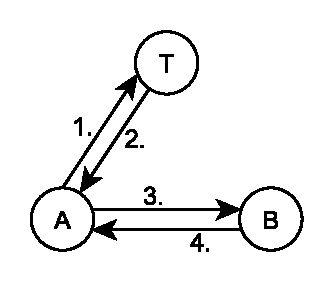
\includegraphics[width=0.5\textwidth]{pic/key_distribution-kerberos}
    \caption{Схема взаимодействия абонентов и доверенного центра в протоколе <<Kerberos>>\label{fig:key_distribution-kerberos}}
\end{figure}

\begin{protocol}
	\item[(1)] $ Alice \to \{ A, B \} \to Trent $
	\item[(2)] $ Trent \to \{ E_A \left( T_T, L, K, B \right), E_B \left( T_T, L, K, A \right) \} \to Alice $
	\item[(3)] $ Alice \to \{ E_B \left( T_T, L, K, A \right), E_K \left( A, T_A \right) \} \to Bob $
	\item[(4)] $ Bob \to \{ E_K \left( T_T + 1 \right) \} \to Alice $
\end{protocol}

Обратите внимание, что на третьем проходе за счёт использования метки времени от доверенного центра $T_T$ вместо случайной метки от Боба $R_B$ позволяет сократить количество проходов на один по сравнению с протоколом Нидхема~---~Шрёдера\index{протокол!Нидхема~---~Шрёдера}. Также наличие метки времени делает ненужным и предварительную генерацию случайной метки Алисой и её передачу на первом шаге.

Метка времени $T_A$ в сообщении $E_K \left( A, T_A \right)$ позволяет Бобу убедиться, что Алиса владеет текущим сессионным ключом $K$. Если расшифрованная метка $T_A$ сильно отличается от текущего времени, значит либо этот пакет из другого сеанса протокола, либо не от Алисы вообще.

Интересно отметить, что пакеты $E_A \left( T_T, L, K, B \right)$ и $E_B \left( T_T, L, K, A \right)$ одинаковы по своему формату. В некотором смысле их можно назвать сертификатами сессионного ключа для Алисы и Боба. Причём все подобные пары пакетов можно сгенерировать заранее (например, в начале дня), выложить на общедоступный ресурс, предоставить в свободное использование и выключить доверенный центр (он своё дело уже сделал -- сгенерировав эти пакеты). И до момента времени $T_T + L$ этими <<сертификатами>> можно пользоваться. Но только если вы являетесь одной из допустимых пар абонентов. Конечно, эта идея непрактична -- ведь количество таких пар растёт как квадрат от числа абонентов. Однако интересен тот факт, что подобные пакеты можно сгенерировать заранее. Эта идея нам пригодится при рассмотрении инфраструктуры открытых ключей (\langen{public key infrastructure, PKI}).

\index{протокол!Kerberos|)}

\section{Pretty Good Privacy}
\selectlanguage{russian}

В качестве примера передачи файлов по сети с обеспечением аутентификации, конфиденциальности и целостности рассмотрим систему PGP (\langen{Pretty Good Privacy}), разработанную Филом Циммерманном (\langen{Phil Zimmermann}) в 1991 г. Изначально система предлагалась к использованию для защищённой передачи электронной почты. Стандартом PGP является OpenPGP. Примерами реализации стандарта OpenPGP являются GNU Privacy Guard (GPG) и netpgp, разработанные в рамках проектов GNU и NetBSD соответственно.

Каждый пользователь обладает одной или несколькими парами из закрытого и открытого ключей. Ключи используются как для расшифрования получаемых пользователем сообщений, так и для генерации электронных подписей отправляемых сообщений. Также пользователь хранит открытые ключи других участников системы, чтобы иметь возможность отправлять им зашифрованные сообщения и аутентифицировать отправителей принимаемых сообщений.

В системе PGP каждое передаваемое сообщение подписывается закрытым ключом отправителя, затем сообщение шифруется блочной криптосистемой на случайно выбранном секретном сеансовом ключе. Сам сеансовый ключ шифруется криптосистемой с открытым ключом на открытом ключе получателя.

Свои закрытые ключи отправитель хранит в зашифрованном виде. Набор ключей называется связкой закрытых ключей. Шифрование закрытых ключей в связке производится симметричным шифром\index{шифр!симметричный}, ключом которого является функция от пароля, вводимого пользователем. Шифрование закрытых ключей, хранимых на компьютере, является стандартной практикой для защиты от утечки, например, в случае взлома ОС, утери ПК и~т.\,д.

Набор открытых ключей других пользователей называется связкой открытых ключей.

\begin{figure}[!ht]
	\centering
	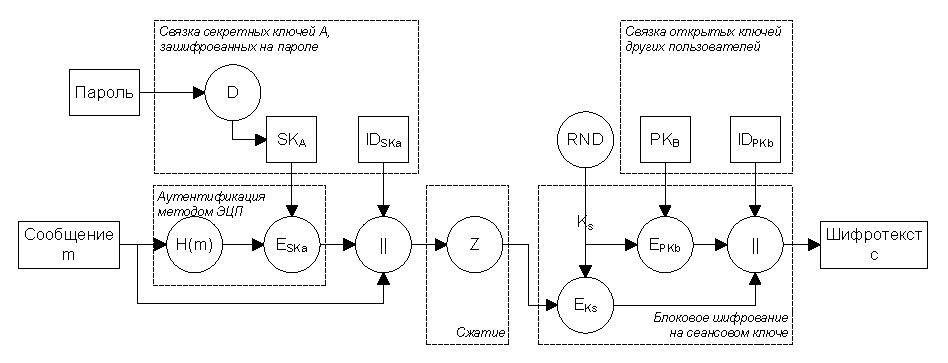
\includegraphics[width=0.9\textwidth]{pic/pgp}
	\caption{Схема обработки сообщения в PGP\label{fig:pgp}}
\end{figure}

На рис.~\ref{fig:pgp} представлена схема обработки сообщения в PGP для передачи от $A$ к $B$. Использование аутентификации, сжатия и блочного шифрования является опциональным. Обозначения на рисунке следующие:
\begin{itemize}
    \item Пароль -- пароль, вводимый отправителем для расшифрования связки своих закрытых ключей;
    \item $D$ -- расшифрование блочной криптосистемы для извлечения секретного ключа ЭП отправителя;
    \item $SK_A$ -- закрытый ключ ЭП отправителя;
    \item $ID_{SKa}$ -- идентификатор ключа ЭП отправителя, по которому получатель определяет, какой ключ из связки открытых ключей использовать для проверки подписи;
    \item $m$ -- сообщение (файл) для передачи;
    \item $h(m)$ -- криптографическая хэш-функция;
    \item $E_{SKa}$ -- схема ЭП на секретном ключе $SK_A$;
    \item $\|$ -- конкатенация битовых строк;
    \item $Z$ -- сжатие сообщения алгоритмом компрессии;
    \item $RND$ -- криптографический генератор псевдослучайной последовательности;
    \item $K_s$ -- сгенерированный псевдослучайный сеансовый ключ;
    \item $E_{Ks}$ -- блочное шифрование на секретном сеансовом ключе $K_s$;
    \item $PK_B$ -- открытый ключ получателя;
    \item $ID_{PKb}$ -- идентификатор открытого ключа получателя, по которому получатель определяет, какой ключ из связки закрытых ключей использовать для расшифрования сеансового ключа;
    \item $E_{PKb}$ -- шифрование сеансового ключа криптосистемой с открытым ключом на открытом ключе $B$;
    \item $c$ -- зашифрованное подписанное сообщение.
\end{itemize}


\section{Протокол SSL/TLS}\index{протокол!SSL/TLS}
\selectlanguage{russian}

Протокол SSL (\langen{Secure Sockets Layer}) был разработан компанией Netscape. Начиная с версии 3, протокол развивается как открытый стандарт TLS (\langen{Transport Layer Security}). Протокол SSL/TLS обеспечивает защищённое соединение по незащищённому каналу связи на прикладном уровне модели TCP/IP. Протокол встраивается между прикладным и транспортным уровнями стека протоколов TCP/IP. Для обозначения <<новых>> протоколов, полученных с помощью инкапсуляции прикладного уровня (HTTP\index{протокол!HTTP}, FTP\index{протокол!FTP}, SMTP\index{протокол!SMTP}, POP3\index{протокол!POP3}, IMAP\index{протокол!IMAP} и~т.\,д.) в SSL/TLS, к обозначению добавляют суффикс <<S>> (<<Secure>>): HTTPS\index{протокол!HTTPS}, FTPS\index{протокол!FTPS}, POP3S\index{протокол!POP3S}, IMAPS\index{протокол!IMAPS} и~т.\,д.

Протокол обеспечивает следующее:
\begin{itemize}
    \item Одностороннюю или взаимную аутентификацию клиента и сервера по открытым ключам сертификата X.509. В Интернете, как правило, делается \emph{односторонняя} аутентификация веб-сервера браузеру клиента, то есть только веб-сервер предъявляет сертификат (открытый ключ и ЭП к нему от вышележащего УЦ).
    \item Создание сеансовых симметричных ключей для шифрования и кода аутентификации сообщения для передачи данных в обе стороны.
    \item Конфиденциальность\index{конфиденциальность} -- блочное или потоковое шифрование передаваемых данных в обе стороны.
    \item Целостность\index{целостность} -- аутентификацию отправляемых сообщений в обе стороны имитовставкой\index{имитовставка} $\HMAC(K,M)$, описанной ранее.
\end{itemize}

Рассмотрим протокол TLS последней версии 1.2.


\subsection{Протокол <<рукопожатия>>}

Протокол <<рукопожатия>> (\langen{Handshake Protocol}) производит аутентификацию и создание сеансовых ключей между клиентом $C$ и сервером $S$.

\begin{enumerate}
    \item $C \rightarrow S$:
        \begin{enumerate}
            \item ClientHello: ~ 1) URI сервера, ~ 2) одноразовая метка $N_C$\index{одноразовая метка}, ~ 3) поддерживаемые алгоритмы шифрования, кода аутентификации сообщений, хэширования, ЭП и сжатия.
        \end{enumerate}

    \item $C \leftarrow S$:
        \begin{enumerate}
            \item ServerHello: одноразовая метка $N_S$, поддерживаемые сервером алгоритмы.

            После обмена набором желательных алгоритмов сервер и клиент по единому правилу выбирают общий набор алгоритмов.
            \item Server Certificate: сертификат X.509v3 сервера с запрошенным URI (URI нужен в случае нескольких виртуальных веб-серверов с разными URI на одном узле c одним IP-адресом).
            \item Server Key Exchange Message: информация для создания предварительного общего секрета $premaster$ длиной 48 байтов в виде: ~ 1) обмена по протоколу Диффи~---~Хеллмана\index{протокол!Диффи~---~Хеллмана} с клиентом (сервер отсылает $(g, g^a)$), ~ 2)Обмена по другому алгоритму с открытым ключом, ~ 3) разрешения клиенту выбрать ключ.
            \item Электронная подпись к Server Key Exchange Message на ключе сертификата сервера для аутентификации сервера клиенту.
            \item Certificate Request: опциональный запрос сервером сертификата клиента.
            \item Server Hello Done: идентификатор конца транзакции.
        \end{enumerate}

    \item $C \rightarrow S$:
        \begin{enumerate}
            \item Client Certificate: сертификат X.509v3 клиента, если он был запрошен сервером.
            \item Client Key Exchange Message: информация для создания предварительного общего секрета $premaster$ длиной 48 байтов в виде: ~ 1) либо обмена по протоколу Диффи~---~Хеллмана\index{протокол!Диффи~---~Хеллмана} с сервером (клиент отсылает $g^b$, в результате обе стороны вычисляют ключ $premaster = g^{ab}$), ~ 2) либо обмена по другому алгоритму, ~ 3) либо ключа, выбранного клиентом и зашифрованного на открытом ключе из сертификата сервера.
            \item Электронная подпись к Client Key Exchange Message на ключе сертификата клиента для аутентификации клиента серверу (если клиент использует сертификат).
            \item Certificate Verify: результат проверки сертификата сервера.
            \item Change Cipher Spec: уведомление о смене сеансовых ключей.
            \item Finished: идентификатор конца транзакции.
        \end{enumerate}

    \item $C \leftarrow S$:
        \begin{enumerate}
            \item Change Cipher Spec: уведомление о смене сеансовых ключей.
            \item Finished: идентификатор конца транзакции.
        \end{enumerate}
\end{enumerate}

%      http://tools.ietf.org/html/rfc5246#page-37

%      struct {
%          ProtocolVersion client_version;
%          Random random;
%          SessionID session_id;
%          CipherSuite cipher_suites<2..2^16-2>;
%          CompressionMethod compression_methods<1..2^8-1>;
%          select (extensions_present) {
%              case false:
%                  struct {};
%              case true:
%                  Extension extensions<0..2^16-1>;
%          };
%      } ClientHello;

%      struct {
%          ProtocolVersion server_version;
%          Random random;
%          SessionID session_id;
%          CipherSuite cipher_suite;
%          CompressionMethod compression_method;
%          select (extensions_present) {
%              case false:
%                  struct {};
%              case true:
%                  Extension extensions<0..2^16-1>;
%          };
%      } ServerHello;

%      struct {
%          ASN.1Cert certificate_list<0..2^24-1>;
%      } Certificate;

%      struct {
%          select (KeyExchangeAlgorithm) {
%              case dh_anon:
%                  ServerDHParams params;
%              case dhe_dss:
%              case dhe_rsa:
%                  ServerDHParams params;
%                  digitally-signed struct {
%                      opaque client_random[32];
%                      opaque server_random[32];
%                      ServerDHParams params;
%                  } signed_params;
%              case rsa:
%              case dh_dss:
%              case dh_rsa:
%                  struct {} ;
%                 /* message is omitted for rsa, dh_dss, and dh_rsa */
%              /* may be extended, e.g., for ECDH -- see [TLSECC] */
%          };
%      } ServerKeyExchange;

%      struct {
%          ClientCertificateType certificate_types<1..2^8-1>;
%          SignatureAndHashAlgorithm
%            supported_signature_algorithms<2^16-1>;
%          DistinguishedName certificate_authorities<0..2^16-1>;
%      } CertificateRequest;

%      struct {
%          select (KeyExchangeAlgorithm) {
%              case rsa:
%                  EncryptedPreMasterSecret;
%              case dhe_dss:
%              case dhe_rsa:
%              case dh_dss:
%              case dh_rsa:
%              case dh_anon:
%                  ClientDiffieHellmanPublic;
%          } exchange_keys;
%      } ClientKeyExchange;

%      struct {
%           digitally-signed struct {
%               opaque handshake_messages[handshake_messages_length];
%           }
%      } CertificateVerify;

%      struct {
%          opaque verify_data[verify_data_length];
%      } Finished;

Одноразовая метка $N_C$ состоит из 32 байтов. Первые 4 байта содержат текущее время (gmt\_unix\_time), оставшиеся байты -- псевдослучайную последовательность, которую формирует криптографически стойкий генератор псевдослучайных чисел.

Предварительный общий секрет $premaster$ длиной 48 байтов вместе с одноразовыми метками используется как инициализирующее значение генератора $PRF$ для получения общего секрета $master$, тоже длиной 48 байтов:
    \[ master = PRF(premaster, ~\text{текст \textquotedblleft master secret\textquotedblright}, ~ N_C + N_S) .\]

И, наконец, уже из секрета $master$ таким же способом генерируется 6 окончательных сеансовых ключей, следующих друг за другом в битовой строке:
    \[ \{ (K_{E,1} ~\|~ K_{E,2}) ~\|~ (K_{\MAC,1} ~\|~ K_{\MAC,2}) ~\|~ (IV_1 ~\|~ IV_2) \} = \]
        \[ = PRF(master, ~\text{текст \textquotedblleft key expansion\textquotedblright}, ~ N_C + N_S), \]
где ~ $K_{E,1}, ~ K_{E,2}$ -- два ключа симметричного шифрования, ~ $K_{\MAC,1}, ~ K_{\MAC,2}$ -- два ключа имитовставки\index{имитовставка}, ~ $IV_1, ~IV_2$ -- два инициализирующих вектора режима сцепления блоков\index{вектор инициализации}. Ключи с индексом 1 используются для коммуникации от клиента к серверу, с индексом 2 -- от сервера к клиенту.


\subsection{Протокол записи}

Протокол записи (\langen{Record Protocol}) определяет формат TLS-пакетов для вложения в TCP-пакеты.

\begin{enumerate}
    \item Исходными сообщениями $M$ для шифрования являются пакеты протокола следующего уровня в модели OSI: HTTP\index{протокол!HTTP}, FTP\index{протокол!FTP}, IMAP\index{протокол!IMAP} и~т.\,д.
    \item Сообщение $M$ разбивается на блоки $m_i$ размером не более 16 кибибайт.
    \item Блоки $m_i$ сжимаются алгоритмом компрессии в блоки $z_i$.
    \item Вычисляется имитовставка\index{имитовставка} для каждого блока $z_i$ и добавляется в конец блоков: $a_i = z_i ~\|~ \HMAC(K_{\MAC}, z_i)$.
    \item Блоки $a_i$ шифруются симметричным алгоритмом с ключом $K_E$ в некотором режиме сцепления блоков с инициализирующим вектором $IV$ в полное сжатое аутентифицированное зашифрованное сообщение $C$.
    \item К шифртексту $C$ добавляется заголовок протокола записи TLS, в результате чего получается TLS-пакет для вложения в TCP-пакет.
\end{enumerate}


\section{Защита IPsec на сетевом уровне}\index{протокол!IPsec|(}
\selectlanguage{russian}

Набор протоколов IPsec (\langen{Internet Protocol Security})~\cite{rfc4301} является неотъемлемой частью IPv6\index{протокол!IPv6} и дополнительным необязательным расширением IPv4. IPsec обеспечивает защиту данных на сетевом уровне IP-пакетов.

IPsec определяет:
\begin{itemize}
    \item первичную аутентификацию сторон и управление сеансовыми ключами (протокол IKE, Internet Key Exchange);\index{протокол!IKE}
    \item шифрование с аутентификацией (протокол ESP, Encapsulating Security Payload);\index{протокол!ESP}
    \item только аутентификацию сообщений (протокол AH, Authentication Header).\index{протокол!AH}
\end{itemize}
Основное (современное) применение этих протоколов состоит в построении VPN\index{протокол!VPN} (Virtual Private Network -- виртуальная частная сеть) при использовании IPsec в так называемом туннельном режиме.

Аутентификация в режимах ESP и AH определяется по-разному. Аутентификация в ESP гарантирует целостность\index{целостность} только зашифрованных полезных данных (пакетов следующего уровня после IP). Аутентификация AH гарантирует целостность всего IP-пакета (за исключением полей, изменяемых в процессе передачи пакета по сети).

\subsection{Протокол создания ключей IKE}

%http://www.ietf.org/rfc/rfc4306.txt

Протокол IKE версии 2 (\langen{Internet Key Exchange})\index{протокол!IKE}~\cite{rfc4306}, по существу, можно описать следующим образом. Пусть $I$ -- инициатор соединения, $R$ -- отвечающая сторона.

Протокол состоит из двух фаз. Первая фаза очень похожа на установление соединения в SSL/TLS: она включает возможный обмен сертификатами $C_I, C_R$ стандарта X.509 для аутентификации (или альтернативную аутентификацию по общему заранее созданному секретному ключу) и создание общих предварительных сеансовых ключей протокола IKE по протоколу Диффи~---~Хеллмана\index{протокол!Диффи~---~Хеллмана}. Сеансовые ключи протокола IKE служат для шифрования и аутентификации сообщений второй фазы. Вторая фаза создаёт сеансовые ключи для протоколов ESP, AH, то есть ключи для шифрования конечных данных. Сообщения второй фазы также используются для смены ранее созданных сеансовых ключей, и в этом случае протокол сразу начинается со второй фазы с применением ранее созданных сеансовых ключей протокола IKE.

\begin{enumerate}
    \item Создание предварительной защищённой связи для протокола IKE и аутентификация сторон.
        \begin{enumerate}
            \item $I \rightarrow R$: ~ $\left(g^{x_I}\right.$, одноразовая метка $N_I$, идентификаторы поддерживаемых криптографических алгоритмов$\left.\right)$.
                % HDR, SAi1, KEi, Ni   -->

            \item $I \leftarrow R$: ~$\left(g^{x_R}\right.$, одноразовая метка $N_R$, идентификаторы выбранных алгоритмов, запрос сертификата $C_I\left.\right)$.
                % <--    HDR, SAr1, KEr, Nr, [CERTREQ]

                Протокол Диффи~---~Хеллмана\index{протокол!Диффи~---~Хеллмана} оперирует с генератором $g=2$ в группе $\Z_p^*$ для одного из двух фиксированных $p$ длиной 768 или 1024 бита. После обмена элементами $g^{x_I}$ и $g^{x_R}$ обе стороны обладают общим секретом $g^{x_I x_R}$.

                Одноразовые метки $N_I, N_R$ созданы криптографическим генератором псевдослучайных чисел $PRF$.

                После данного сообщения стороны договорились об используемых алгоритмах и создали общие сеансовые ключи:
                    \[ seed = PRF(N_i ~\|~ N_r, ~g^{x_I x_R}), \]
                    \[ \{ K_d \| Ka_I \| Ka_R \| Ke_I \| Ke_R
                        % \| Kp_I \| Kp_R
                        \} = PRF(seed, ~ N_i ~\|~ N_r), \]
                где $Ka_I, Ka_R$ -- ключи кода аутентификации для связи в обоих направлениях, ~ $Ke_I, Ke_R$ -- ключи шифрования сообщений для двух направлений, ~ $K_d$ -- инициирующее значение генератора $PRF$ для создания сеансовых ключей окончательной защищённой связи, ~ функцией $PRF(x)$ обозначается выход генератора с инициализирующим значением $x$.
                %$Kp_I, Kp_R$ --  which areused when generating an AUTH payload.

                При дальнейшем обмене данными сообщения шифруются алгоритмом AES\index{шифр!AES} в режиме CBC со случайно выбранным инициализирующим вектором $IV$ на сеансовых ключах $Ke$ и аутентифицируются имитовставкой\index{имитовставка} на ключах $Ka$. Введём обозначения для шифрования сообщения $m$ со сцеплением блоков $E_{Ke_X}(m)$, и совместного шифрования, и добавления кода аутентификации сообщений $\langle m \rangle_X$ для исходящих данных от стороны $X$:
                    \[  E_{Ke_X}(m) = IV ~\|~ E_{Ke_X}(IV ~\|~ m), \]
                    \[  \langle m \rangle_X = E_{Ke_X}(m) ~\|~ \HMAC(Ka_X, ~ E_{Ke_X}(m)). \]

            \item $I \rightarrow R$: ~ $\langle ID_I, ~ C_I, ~\text{запрос сертификата}~ C_R, ~ ID_R, ~ A_I \rangle_I$.
                % HDR, SK {IDi, [CERT,] [CERTREQ,] [IDr,] AUTH, SAi2, TSi, TSr}     -->

                По значениям идентификаторов $ID_I, ID_R$ сторона $R$ проверяет знание стороной $I$ ключей $Ke, Ka$.

                Поле $A_I$ обеспечивает аутентификацию стороны $I$ стороне $R$ одним из двух способов. Если используются сертификаты, то $I$ показывает, что обладает закрытым ключом, парным открытому ключу сертификата $C_I$, подписывая сообщение $data$:
                    \[ A_I = \textrm{ЭП}(data). \]
                Сторона $R$ также проверяет сертификат $C_I$ по цепочке до доверенного сертификата верхнего уровня.

                Второй вариант аутентификации -- по общему секретному симметричному ключу аутентификации $K_{IR}$, который заранее был создан $I$ и $R$, как в Kerberos. Сторона $I$ показывает, что знает общий секрет, вычисляя
                    \[ A_I = PRF( PRF(K_{IR}, ~ \text{текст ''Key Pad for IKEv2''}), ~ data). \]
                Сторона $R$ сравнивает присланное значение $A_I$ с вычисленным и убеждается, что $I$ знает общий секрет.

                Сообщение $data$ -- это открытое сообщение данной транзакции, за исключением нескольких полей.

            \item $I \leftarrow R$: ~ $\langle ID_R, ~ C_R, ~ A_R \rangle_R$.
                % HDR, SK {IDr, [CERT,] AUTH, SAr2, TSi, TSr}

                Производится аутентификация стороны $R$ стороной $I$ аналогичным образом.
        \end{enumerate}

    \item Создание защищённой связи для протоколов ESP, AH, то есть ключей шифрования и кодов аутентификации конечных полезных данных. Фаза повторяет первые две транзакции первой фазы с созданием ключей по одноразовой метке $N'$ и протоколу Диффи~---~Хеллмана\index{протокол!Диффи~---~Хеллмана} с закрытыми ключами $x'$.
        \begin{enumerate}
            \item $I \rightarrow R$: ~ $\langle g^{x'_I}$, одноразовая метка $N'_I$, поддерживаемые алгоритмы для ESP, AH$\rangle_I$.
                % HDR, SK {[N], SA, Ni, [KEi], [TSi, TSr]}             -->
            \item $I \rightarrow R$: ~ $\langle g^{x'_R}$, одноразовая метка $N'_R$, выбранные алгоритмы для ESP, AH$\rangle_R$.
                % <--    HDR, SK {SA, Nr, [KEr], [TSi, TSr]}
        \end{enumerate}
        По окончании второй фазы обе стороны имеют общие секретные ключи $Ke, Ka$ для шифрования и коды аутентификации в двух направлениях, от стороны $I$ и от стороны $R$:
            \[ \{Ka'_I ~\|~ Ka'_R ~\|~ Ke'_I ~\|~ Ke'_R \} = PRF(K_d, ~ g^{x'_I x'_R} ~\|~ N'_I ~\|~ N'_r). \]
\end{enumerate}

Итогом работы протокола IKE является набор сеансовых ключей для шифрования $Ke'_I, ~ Ke'_R$ и кодов аутентификации $Ka'_I, ~ Ka'_R$ в протоколах ESP и AH.


\subsection{Таблица защищённых связей}

\emph{Защищённая связь} (\langen{Security Association, SA}) является \emph{однонаправленной} от отправителя к получателю и характеризуется тремя основными параметрами:
\begin{itemize}
    \item индексом параметров защиты -- уникальным 32-битовым числом, входящим в заголовок ESP- и AH-пакетов;
    \item IP-адресом стороны-отправителя;
    \item идентификатором применения ESP- или AH-протокола.
\end{itemize}

Защищённые связи хранятся в таблице защищённых связей со следующими полями:
\begin{itemize}
    \item счётчик порядкового номера, входит в заголовок ESP- и AH-пакетов;
    \item окно защиты от воспроизведения -- скользящий буфер порядковых номеров пакетов для защиты от пропуска и повтора пакетов;
    \item информация протокола ESP и AH -- алгоритмы, ключи, время действия ключей;
    \item режим протокола: транспортный или туннельный.
\end{itemize}

По индексу параметров защиты, находящемуся в заголовке ESP- и AH-пакетов, получатель из таблицы защищённых связей извлекает параметры (названия алгоритмов, ключи и~т.\,д.), производит проверки счётчиков, аутентифицирует и расшифровывает вложенные данные для принятого IP-пакета.
%Или создаёт зашифрованный аутентифицированный IP-пакет, который включает индекс параметров защиты, чтобы получатель мог из своей таблицы защищённых связей извлечь ключи для аутентификации и расшифрования.

Протоколы ESP и AH можно применять к IP-пакету в трёх вариантах:
\begin{itemize}
    \item только ESP-протокол;
     \item только AH-протокол;
    \item последовательное применение ESP- и AH-протоколов.
\end{itemize}
Подчеркнём, что только AH-протокол гарантирует целостность\index{целостность} всего IP-пакета, поэтому для организации виртуальной сети VPN\index{сеть!виртуальная частная}, как правило, применяется третий вариант (последовательно ESP- и AH-протоколы).


\subsection{Транспортный и туннельный режимы}

Протоколы ESP, AH могут применяться в транспортном режиме, когда исходный IP-пакет расширяется заголовками и концевиками протоколов ESP, AH, или в туннельном режиме, когда весь IP-пакет вкладывается в новый IP-пакет, который включает заголовки и концевики ESP, AH.

Новый IP-пакет в туннельном режиме может иметь другие IP-адреса, отличные от оригинальных. Именно это свойство используется для построения виртуальных частных сетей (\langen{Virtual Private Network, VPN})\index{сеть!виртуальная частная}. IP-адресом нового пакета является IP-адрес IPsec-шлюза виртуальной сети. IP-адрес вложенного пакета является локальным адресом виртуальной сети. IPsec-шлюз производит преобразование IPsec-пакетов в обычные IP-пакеты виртуальной сети и наоборот.

Схемы транспортного и туннельного режимов показаны ниже отдельно для ESP- и AH-протоколов.


\subsection{Протокол шифрования и аутентификации ESP}

Протокол ESP\index{протокол!ESP} определяет шифрование и аутентификацию вложенных в IP-пакет сообщений в формате, показанном на рис.~\ref{fig:ipsec-esp}.

\begin{figure}[!ht]
	\centering
	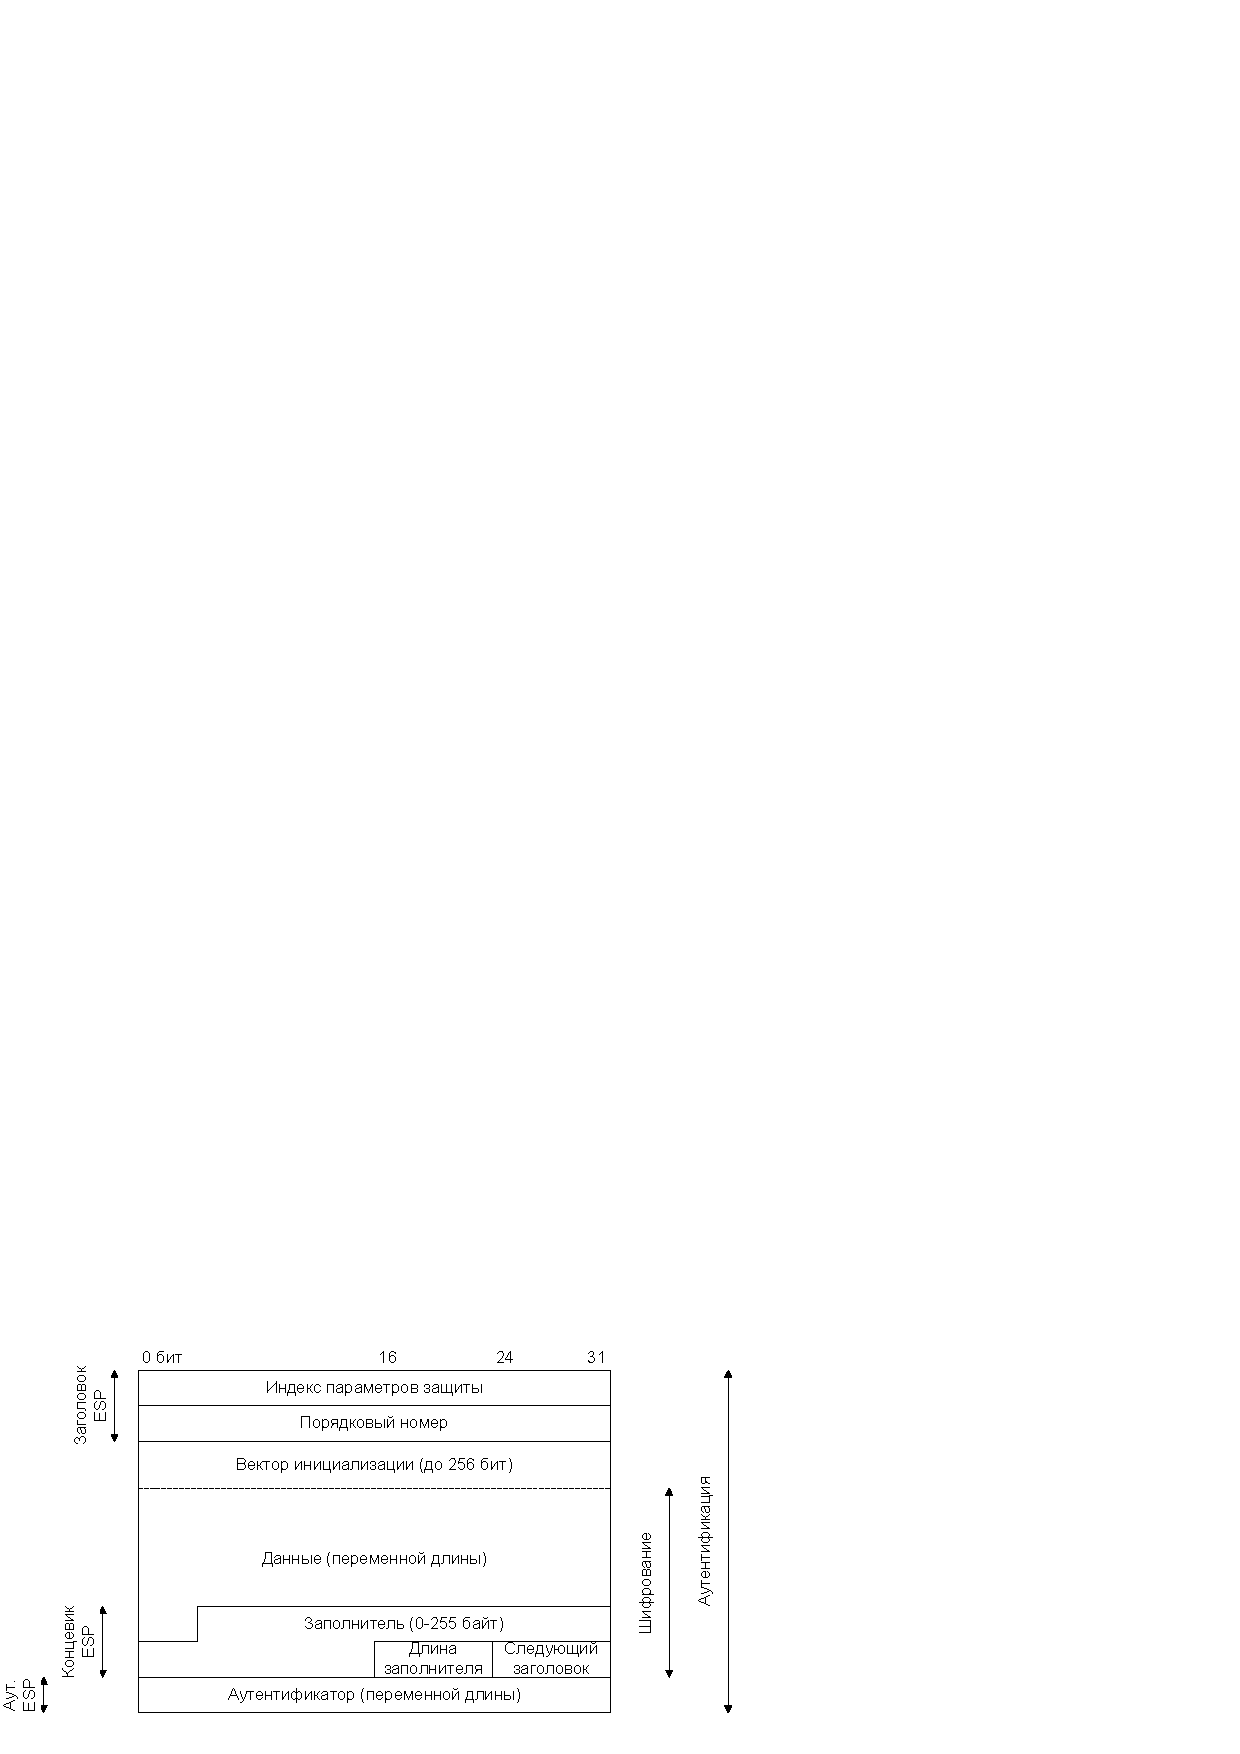
\includegraphics[width=0.9\textwidth]{pic/ipsec-esp}
	\caption{Формат ESP-пакета\label{fig:ipsec-esp}}
\end{figure}

Шифрование вложенных данных производится в режиме CBC алгоритмом AES на ключе $Ke'$ с псевдослучайным вектором инициализации IV, вставленным перед зашифрованными данными.

Аутентификатор сообщения определяется как усечённое до 96 бит значение $\HMAC(Ka', m)$, вычисленное стандартным способом.

На рис.~\ref{fig:ipsec-esp-modes} показано применение протокола в транспортном и туннельном режимах.

\begin{figure}[!ht]
	\centering
	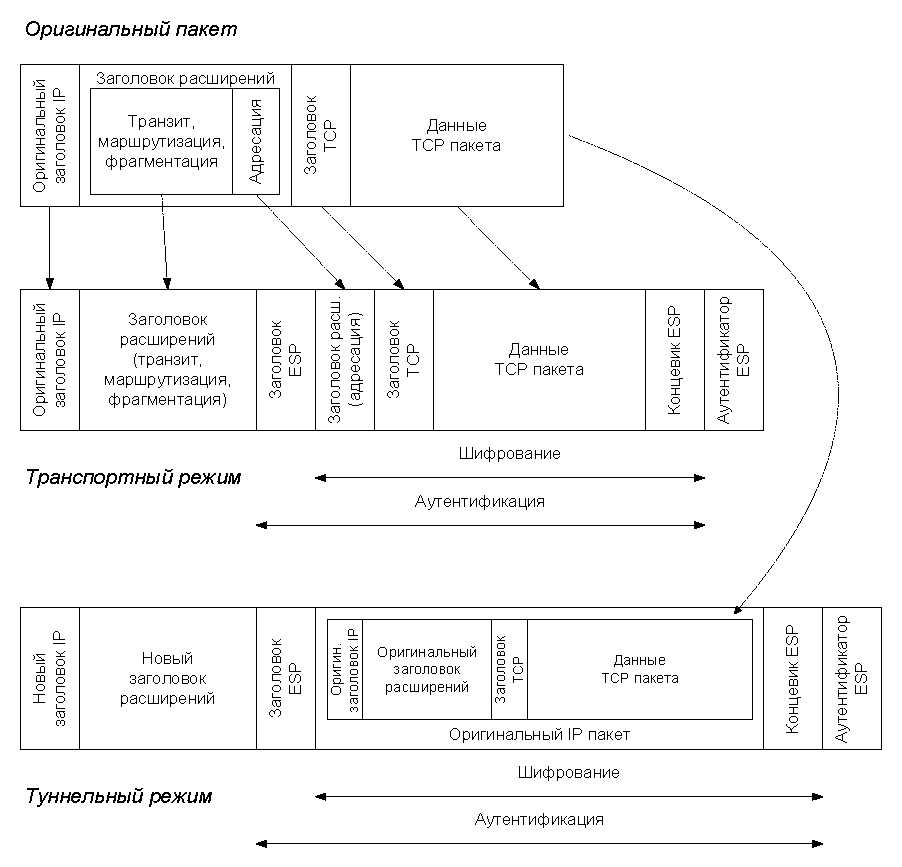
\includegraphics[width=0.9\textwidth]{pic/ipsec-esp-modes}
	\caption{Применение ESP протокола к пакету IPv6\label{fig:ipsec-esp-modes}}
\end{figure}


\subsection{Протокол аутентификации AH}

Протокол AH определяет аутентификацию всего IP-пакета в формате, показанном на рис.~\ref{fig:ipsec-ah}.

\begin{figure}[!ht]
	\centering
	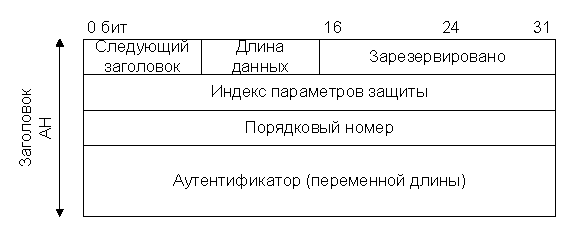
\includegraphics[width=0.7\textwidth]{pic/ipsec-ah}
	\caption{Заголовок AH пакета\label{fig:ipsec-ah}}
\end{figure}

Аутентификатор сообщения определяется так же, как и в протоколе ESP -- усечённое до 96 бит значение $\HMAC(Ka', m)$, вычисленное стандартным способом.

На рис.~\ref{fig:ipsec-ah-modes} показано применение протокола в транспортном и туннельном режимах.

\begin{figure}[!ht]
	\centering
	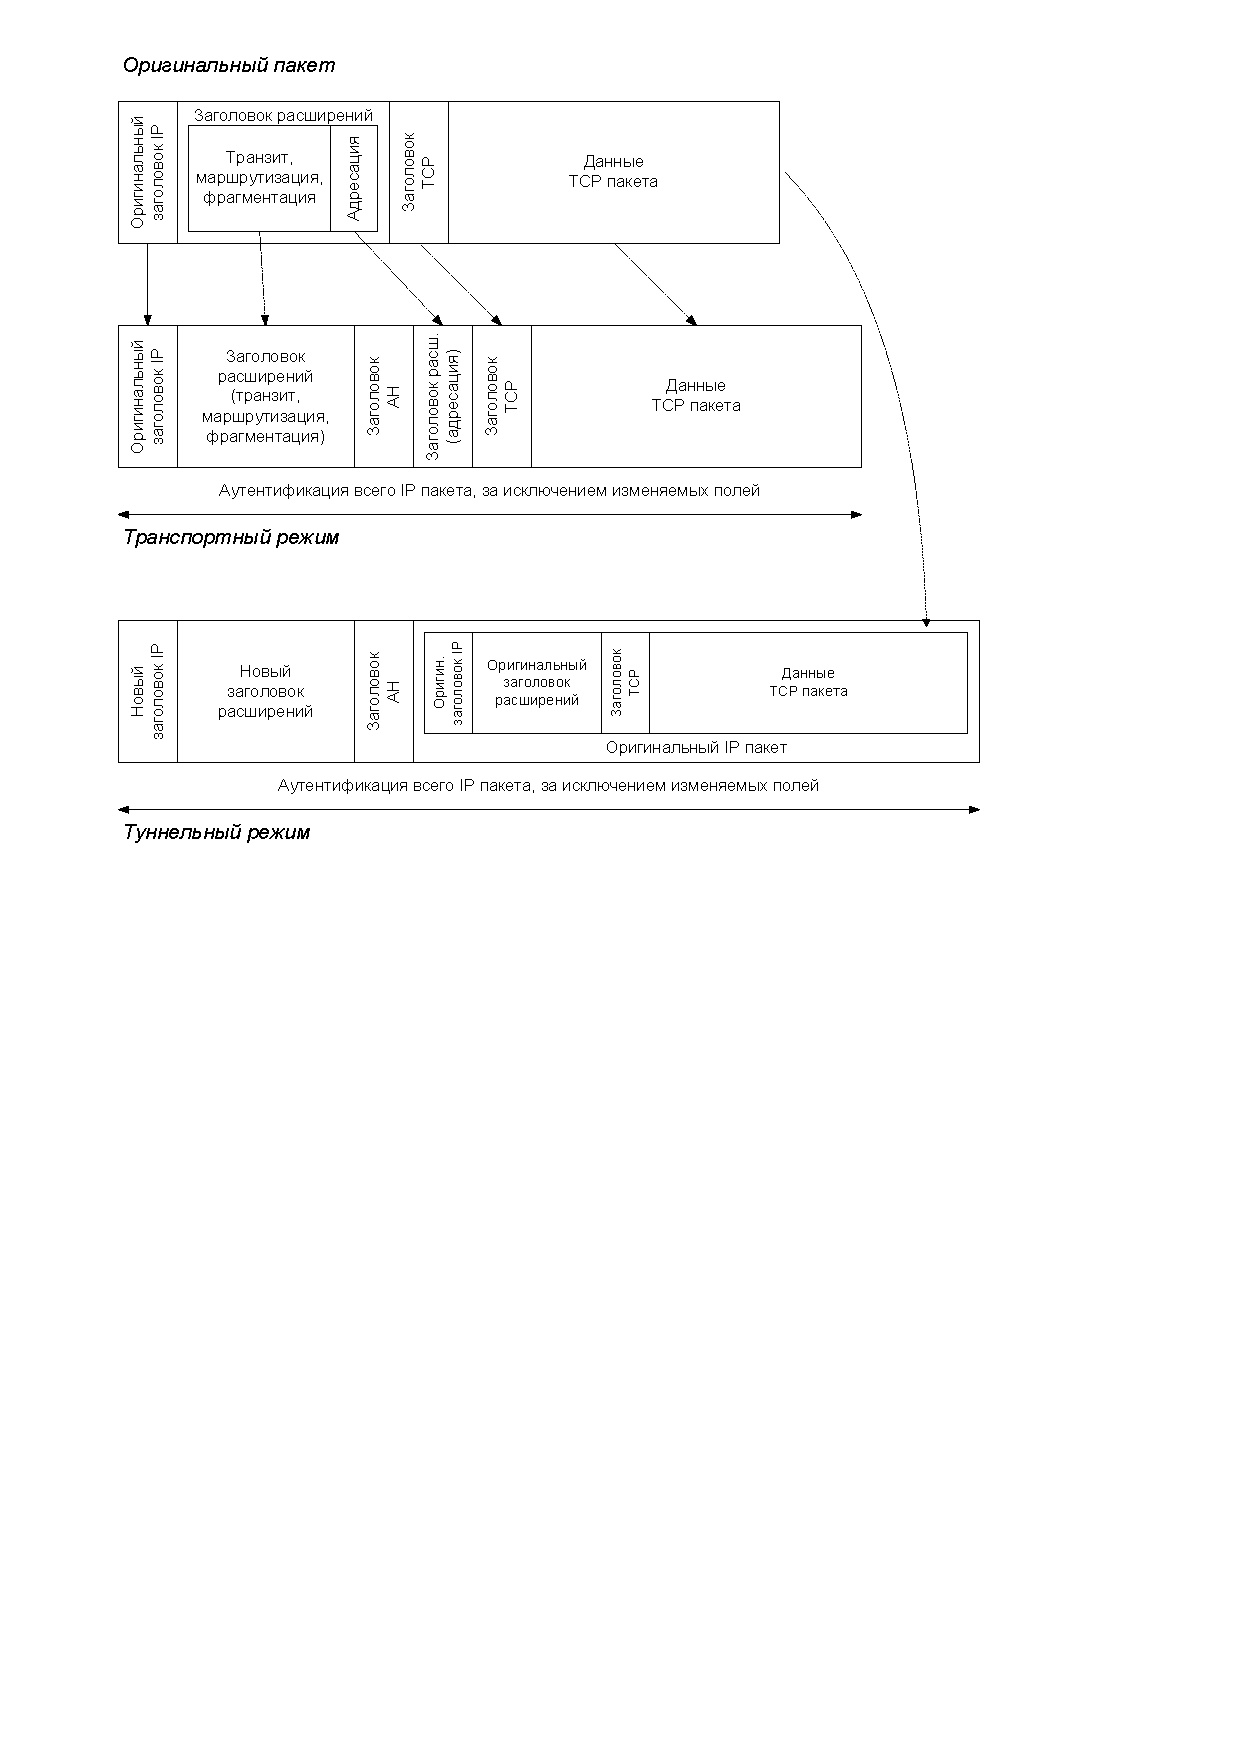
\includegraphics[width=0.9\textwidth]{pic/ipsec-ah-modes}
	\caption{Применение протокола AH к пакету IPv6\label{fig:ipsec-ah-modes}}
\end{figure}

\index{протокол!IPsec|)}

\section[Защита персональных данных в мобильной связи]{Защита персональных данных в \protect\\ мобильной связи}

\subsection{GSM (2G)}
\selectlanguage{russian}

Регистрация телефона в сети GSM построена с участием трёх сторон: SIM-карты мобильного устройства, базовой станции и центра аутентификации. SIM-карта и центр аутентификации обладают общим секретным 128-битным ключом $K_i$. Вначале телефон сообщает базовой станции уникальный идентификатор SIM-карты IMSI открытым текстом. Базовая станция запрашивает в центре аутентификации для данного IMSI набор параметров для аутентификации. Центр генерирует псевдослучайное 128-битовое число $\textrm{RAND}$ и алгоритмами A3\index{алгоритм!A3} и A8\index{алгоритм!A8} создаёт симметричный 54-битовый ключ $K_c$ и 32-битовый аутентификатор $\textrm{RES}$. Базовая станция передаёт мобильному устройству число $\textrm{RAND}$ и ожидает результата вычисления SIM-картой числа $\textrm{XRES}$, которое должно совпасть с $\textrm{RES}$ в случае успешной аутентификации. Схема аутентификации показана на рис.~\ref{fig:gsm2}.

\begin{figure}[!ht]
	\centering
	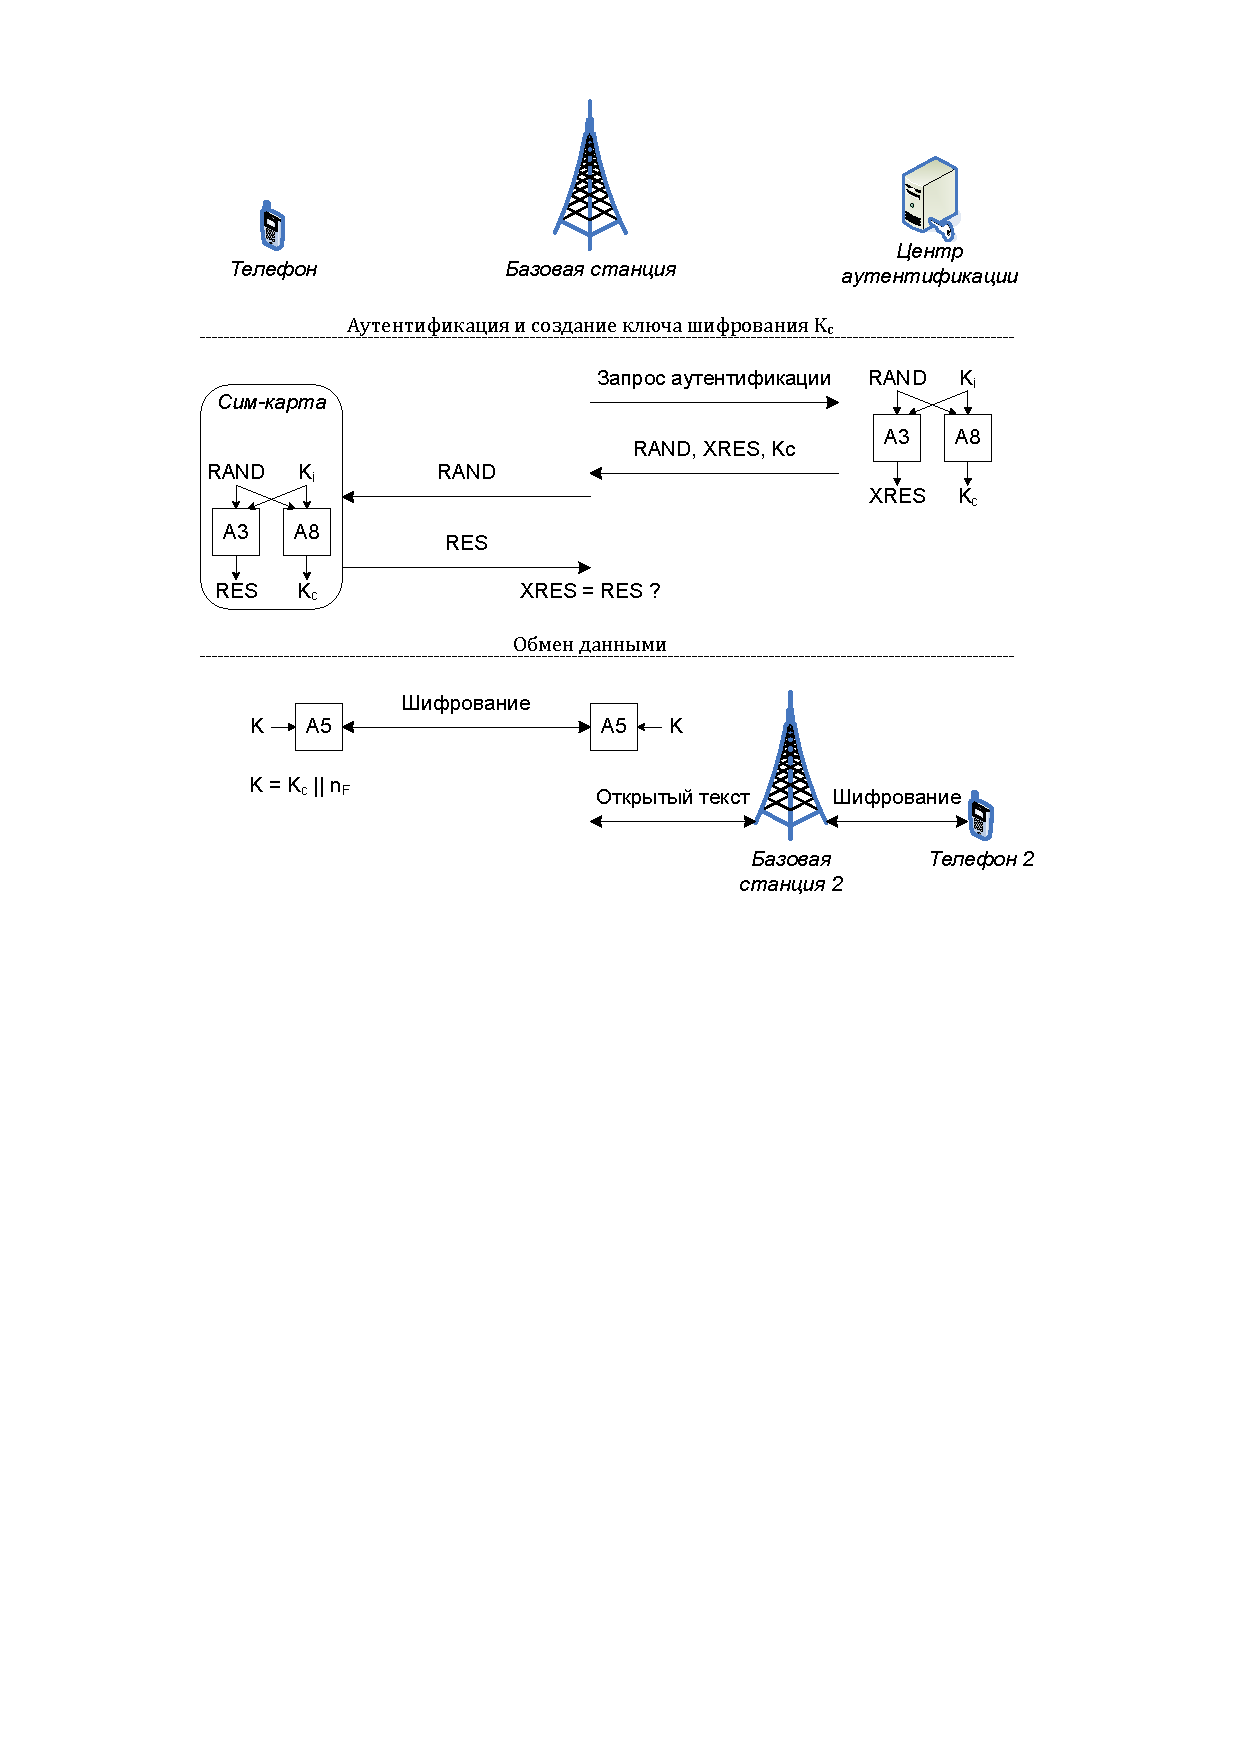
\includegraphics[width=0.85\textwidth]{pic/gsm2}
	\caption{Односторонняя аутентификация и шифрование в GSM\label{fig:gsm2}}
\end{figure}

Все вычисления для аутентификации выполняет SIM-карта. Ключ $K_c$ далее используется для создания ключа шифрования каждого фрейма $K = K_c ~\|~ n_F$, где $n_F$~--~22-битовый номер фрейма. Шифрование выполняет уже само мобильное устройство. Алгоритм шифрования фиксирован в каждой стране и выбирается из семейства алгоритмов A5\index{шифр!A5} (A5/1, A5/2, A5/3). В GSM применяется либо шифр A5/1 (используется в России), либо A5/2. Шифр A5/3 применяется уже в сети UMTS.

Аутентификация в сети GSM односторонняя. При передаче данных не используются проверка целостности и аутентификация сообщений. Передача данных между базовыми станциями происходит в открытом незашифрованном виде. Алгоритмы шифрования A5/1 и A5/2 нестойкие, количество операций для взлома A5/1~--~$2^{40}$, A5/2~--~$2^{16}$. Кроме того, длина ключа $K_c$ всего 54 бита. Передача в открытом виде уникального идентификатора IMSI позволяет однозначно определить абонента.


\subsection{UMTS (3G)}
\selectlanguage{russian}

В третьем поколении мобильных сетей, называемом UMTS, защищённость немного улучшена. Общая схема аутентификации (рис.~\ref{fig:gsm3}) осталась примерно такой же, как и в GSM. Жирным шрифтом на рисунке выделены новые добавленные элементы по сравнению с GSM.
\begin{enumerate}
    \item Производится взаимная аутентификация SIM-карты и центра аутентификации по токенам $\textrm{RES}$ и $\MAC$.
    \item Добавлены проверка целостности и аутентификация данных (имитовставка\index{имитовставка}).
    \item Используются новые алгоритмы создания ключей, шифрования и имитовставки\index{имитовставка}.
    \item Добавлены счётчики на SIM-карте $\textrm{SQN}_{\textrm{T}}$ и в центре аутентификации $\textrm{SQN}_{\textrm{Ц}}$ для защиты от атак воспроизведения. Значения увеличиваются при каждой попытке аутентификации и должны примерно совпадать.
    \item Увеличена длина ключа шифрования до 128 бит.
\end{enumerate}

\begin{figure}[!ht]
	\centering
	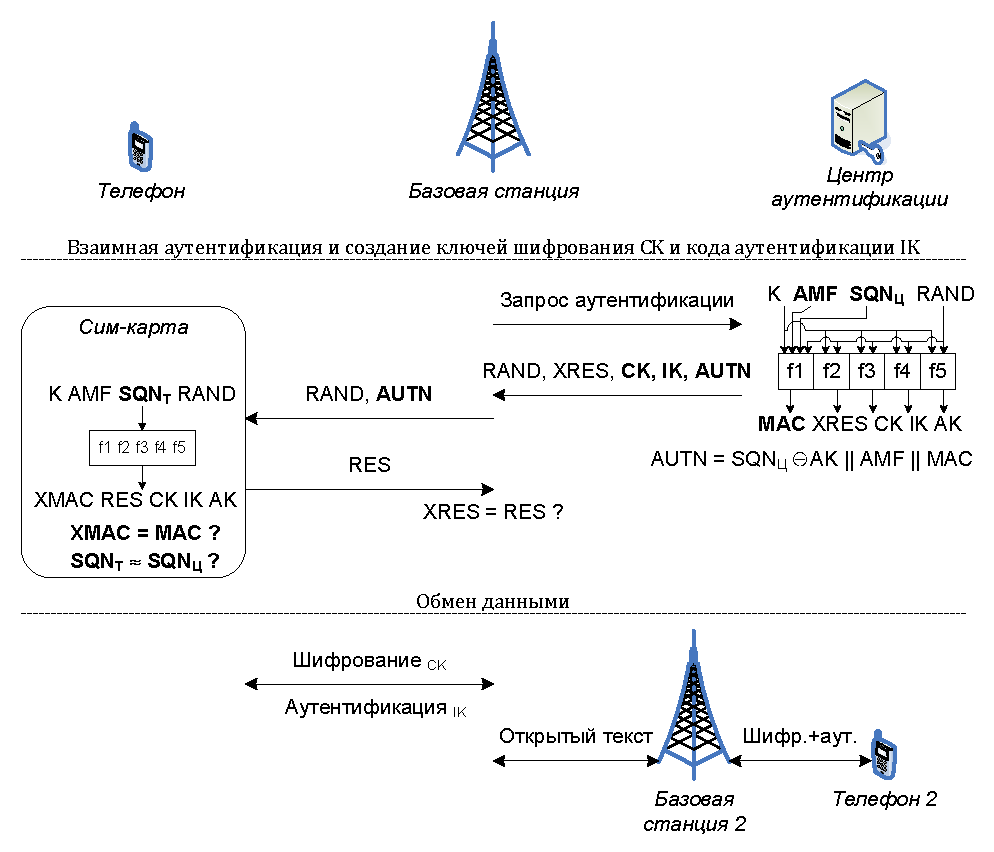
\includegraphics[width=\textwidth]{pic/gsm3}
	\caption{Взаимная аутентификация и шифрование в UMTS (3G)\label{fig:gsm3}}
\end{figure}

Обозначения на рис.~\ref{fig:gsm3} следующие:
\begin{itemize}
    \item $K$ -- общий секретный 128-битовый ключ SIM-карты и центра аутентификации;
    \item $\textrm{RAND}$ -- 128-битовое псевдослучайное число, создаваемое центром аутентификации;
    \item $\textrm{SQN}_{\textrm{T}}, \textrm{SQN}_{\textrm{Ц}}$ -- 48-битовые счётчики для защиты от атак воспроизведения;
    \item $\textrm{AMF}$ -- 16-битовое значение окна для проверки синхронизации счётчиков;
    \item $CK, IK, AK$ -- 128-битовые ключи шифрования данных $CK$, кода аутентификации данных $IK$, гаммы значения счётчика $AK$;
    \item $\MAC, \textrm{XMAC}$ -- 128-битовые аутентификаторы центра SIM-карте;
    \item $\textrm{RES}, \textrm{XRES}$ -- 128-битовые аутентификаторы SIM-карты центру;
    \item $\textrm{AUTN}$ -- вектор аутентификации.
\end{itemize}

Алгоритмы $fi$ не фиксированы стандартом и выбираются при реализациях.

Из оставшихся недостатков защиты персональных данных можно перечислить.
\begin{enumerate}
    \item Уникальный идентификатор SIM-карты IMSI по-прежнему передаётся в открытом виде, что позволяет идентифицировать абонентов по началу сеанса регистрации SIM-карты в сети.
    \item Шифрование и аутентификация производятся только между телефоном и базовой станцией, а не между двумя телефонами. Это является необходимым условием для подключения СОРМ (Система технических средств для обеспечения функций оперативно-розыскных мероприятий) по закону <<О связи>>. С другой стороны, это повышает риск нарушения конфиденциальности персональных данных.
    \item Алгоритм шифрования данных A5/3 (KASUMI) на 128-битовом ключе теоретически взламывается атакой на основе известного открытого текста для 64 MB данных с использованием 1 GiB памяти $2^{32}$ операциями (2 часа на обычном ПК).
\end{enumerate}


%\section{Беспроводная сеть Wi-Fi}
%\subsection{WPA-PSK2, 802.11n, Radix?}
%\subsection{Wimax 802.16(?)}

\chapter{Аутентификация пользователя}


\section{Многофакторная аутентификация}

Для защищённых приложений применяется \emph{многофакторная} аутентификация одновременно по факторам различной природы:
\begin{enumerate}
    \item Свойство, которым обладает субъект. Например: биометрия, природные уникальные отличия (лицо, радужная оболочка глаз, папиллярные узоры, последовательность ДНК).
    \item Знание -- информация, которую знает субъект. Например: пароль, PIN (Personal Identification Number).
    \item Владение -- вещь, которой обладает субъект. Например: электронная или магнитная карта, флэш-память.
%    \item Факторы присвоения. Например, номер машины, RFID-метка.
\end{enumerate}

В обычных массовых приложениях из-за удобства использования применяется аутентификация только по \emph{паролю}\index{пароль}, который является общим секретом пользователя и информационной системы. Биометрическая аутентификация по отпечаткам пальцев применяется существенно реже. Как правило, аутентификация по отпечаткам пальцев является дополнительным, а не вторым обязательным фактором (тоже из-за удобства её использования).

%Так же явно или неявно используется аутентификация по факторам:
%\begin{enumerate}
%    \item Социальная сеть. Доверие к индивидууму в личном или интернет общении, на основании общих связей.
%    \item Географическое положение. Например, для проверки оплаты товаров по кредитной карте.
%    \item Время. Доступ к сервисам или местам только в определённое время.
%    \item И др.
%\end{enumerate}


\section[Энтропия и криптостойкость паролей]{Энтропия и криптостойкость \protect\\ паролей}

Стандартный набор символов паролей, которые можно набрать на клавиатуре, используя английские буквы и небуквенные символы, состоит из $D=94$ символов. При длине пароля $L$ символов и предположении равновероятного использования символов энтропия паролей равна
    \[ H = L \log_2 D. \]

Клод Шеннон, исследуя энтропию символов английского текста, изучал вероятность успешного предсказания людьми следующего символа по первым нескольким символам слов или текста. В результате Шеннон получил оценку энтропии первого символа $s_1$ текста порядка $H(s_1) \approx 4{,}6$--$4{,}7$ бит/символ и оценки энтропий последующих символов, постепенно уменьшающиеся до $H(s_9) \approx 1{,}5$ бит/символ для 9-го символа. Энтропия для длинных текстов литературных произведений получила оценку $H(s_\infty) \approx 0{,}4$ бит/символ.

Статистические исследования баз паролей показывают, что наиболее часто используются буквы <<a>>, <<e>>, <<o>>, <<r>> и цифра <<1>>.

NIST (Национальный институт стандартов и технологий США, \langen{National Institute of Standards and Technology})  использует следующие рекомендации для оценки энтропии паролей\index{энтропия!пароля}, создаваемых людьми.
\begin{enumerate}
    \item Энтропия первого символа $H(s_1) = 4$ бит/символ.
    \item Энтропия со 2-го по 8-й символы $H(s_{i}) = 2$ бит/символ, $2 \leq i \leq 8$.
    \item Энтропия с 9-го по 20-й символы $H(s_{i}) = 1{,}5$ бит/символ, $9 \leq i \leq 20$.
    \item Энтропия с 21-го символа $H(s_{i}) = 1$ бит/символ, $i \geq 21$.
    \item Проверка композиции на использование символов разных регистров и небуквенных символов добавляет до 6-ти бит энтропии пароля.
    \item Словарная проверка на слова и часто используемые пароли добавляет до 6 бит энтропии для коротких паролей. Для 20-символьных и более длинных паролей прибавка к энтропии -- 0 бит.
\end{enumerate}

Для оценки энтропии пароля нужно сложить энтропии символов $H(s_i)$ и сделать дополнительные надбавки, если пароль удовлетворяет тестам на композицию и отсутствует в словаре.

\begin{table}[!ht]
    \caption{Оценка NIST предполагаемой энтропии паролей\label{tab:password-entropy}}
    \resizebox{\textwidth}{!}{ \begin{tabular}{|c||c|c|c||c|}
        \hline
        \multirow{2}{*}{\parbox{1.5cm}{\medskip \centering Длина пароля, символы}} & \multicolumn{3}{|c||}{\parbox{6cm}{\centering Энтропия паролей пользователей по критериям NIST}} & \multirow{2}{*}{\parbox{3cm}{\centering Энтропия случайных равновероятных паролей}} \\
        \cline{2-4}
        & \parbox{1.5cm}{\centering Без проверок} & \parbox{2cm}{\centering Словарная проверка} & \parbox{3cm}{\centering Словарная и композиционная проверка} & \\
        \hline
        4  & 10 & 14 & 16 & 26.3 \\
        6  & 14 & 20 & 23 & 39.5 \\
        8  & 18 & 24 & 30 & 52.7 \\
        10 & 21 & 26 & 32 & 65.9 \\
        12 & 24 & 28 & 34 & 79.0 \\
        16 & 30 & 32 & 38 & 105.4 \\
        20 & 36 & 36 & 42 & 131.7 \\
        24 & 40 & 40 & 46 & 158.0 \\
        30 & 46 & 46 & 52 & 197.2 \\
        40 & 56 & 56 & 62 & 263.4 \\
        \hline
    \end{tabular} }
\end{table}

В таблице~\ref{tab:password-entropy} приведена оценка NIST на величину энтропии пользовательских паролей в зависимости от их длины, и приведено сравнение с энтропией случайных паролей с равномерным распределением символов из набора в $D=94$ символов клавиатуры. Вероятное число попыток для подбора пароля составляет $O(2^H)$. Из таблицы видно, что по критериям NIST энтропия реальных паролей в 2--4 раза меньше энтропии случайных паролей с равномерным распределением символов.

\example
Оценим общее количество существующих паролей. Население Земли -- 7 млрд. Предположим, что всё население использует компьютеры и Интернет, и у каждого человека по 10 паролей. Общее количество существующих паролей -- $7 \cdot 10^{10} \approx 2^{36}$.

Имея доступ к наиболее массовым интернет-сервисам с количеством пользователей десятки и сотни миллионов, в которых пароли часто хранятся в открытом виде из-за необходимости обновления ПО и, в частности, выполнения аутентификации, мы:
\begin{enumerate}
	\item имеем базу паролей, покрывающую существенную часть пользователей; 
	\item можем статистически построить правила генерирования паролей.
\end{enumerate}

Даже если пароль хранится в защищённом виде, то при вводе пароль, как правило, в открытом виде пересылается по Интернету, и все преобразования пароля для аутентификации осуществляет интернет-сервис, а не веб-браузер. Следовательно, интернет-сервис имеет доступ к исходному паролю.
\exampleend

В 2002 г. был подобран ключ для 64-битного блочного шифра RC5 сетью персональных компьютеров \texttt{distributed.net}, выполнявших вычисления в фоновом режиме. Суммарное время вычислений всех компьютеров -- 1757 дней, было проверено 83\% пространства всех ключей. Это означает, что пароли с оценочной энтропией менее 64 бит, то есть \emph{все пароли} до 40 символов по критериям NIST, могут быть подобраны в настоящее время. Конечно, с оговорками на то, что 1) нет ограничений на количество и частоту попыток аутентификаций, 2) алгоритм генерации вероятных паролей эффективен.

Строго говоря, использование даже 40-символьного пароля для аутентификации или в качестве ключа блочного шифрования является небезопасным.


\subsubsection{Число паролей}

Приведём различные оценки числа паролей, создаваемых людьми. Чаще всего такие пароли основаны на словах или закономерностях естественного языка. В английском языке всего около $1\ 000\ 000 \approx 2^{20}$ слов, включая термины.

%http://www.springerlink.com/content/bh216312577r6w64/fulltext.pdf
%http://www.antimoon.com/forum/2004/4797.htm

Используемые слоги английского языка имеют вид V, CV, VC, CVV, VCC, CVC, CCV, CVCC, CVCCC, CCVCC, CCCVCC, где C -- согласная (consonant), V -- гласная (vowel). 70\% слогов имеют структуру VC или CVC. Общее число слогов $S = 8000 \dots 12000$. Средняя длина слога -- 3 буквы.

Предполагая равновероятное распределение всех слогов английского языка, для числа паролей из $r$ слогов получим верхнюю оценку
    \[ N_1 = S^r = 2^{13 r} \approx 2^{4.3 L_1}. \]
Средняя длина паролей составит:
    \[ L_1 \approx 3 r. \]

Теперь предположим, что пароли могут состоять только из 2--3 буквенных слогов вида CV, VC, CVV, VCC, CVC, CCV с равновероятным распределением символов. Подсчитаем число паролей $N_2$, которые могут быть построены из $r$ таких слогов. В английском алфавите число гласных букв $n_v = 10$, согласных $n_c = 16$, $n = n_v + n_c = 26$. Верхняя оценка числа $r$-слоговых паролей:
    \[ N_2 = (n_c n_v + n_v n_c + n_c n_v n_v + n_v n_c n_c + n_c n_v n_c + n_c n_c n_v)^r \approx \]
        \[ \approx \left( n_c n_v(3 n_c + n_v) \right)^r, \]
    \[ N_2 \approx \left( \frac{n^3}{2} \right)^r \approx 2^{13 r} \approx 2^{4.3 L_2}. \]
Средняя длина паролей:
    \[ L_2 = \frac{n_c n_v(2 + 2 + 3 n_v + 3 n_c + 3 n_c + 3 n_c)}{n_c n_v (1 + 1 + n_v + n_c + n_c + n_c)} \cdot r \approx 3 r. \]

Как видно, в обоих предположениях получились одинаковые оценки для числа и длины паролей.

Подсчитаем верхние оценки числа паролей из $L$ символов, предполагая равномерное распределение символов из алфавита мощностью $D$ символов: a) $D_1 = 26$ строчных букв, б) все $D_2 = 94$ печатных символа клавиатуры (латиница и небуквенные символы):
    \[ N_3 = D_1^L \approx 2^{4.7 L}, \]
    \[ N_4 = D_2^L \approx 2^{6.6 L}. \]

\begin{table}[!ht]
    \caption{Различные верхние оценки числа паролей\label{tab:password-number}}
    \resizebox{\textwidth}{!}{ \begin{tabular}{|c||c|c|c|}
        \hline
        \multirow{2}{*}{\parbox{1.5cm}{\medskip\medspace \centering Длина пароля}} & \multicolumn{3}{|c|}{Число паролей} \\
        \cline{2-4}
            & \parbox{3.5cm}{\medspace \centering На основе слоговой композиции} &
            \parbox{3cm}{\medspace\centering Алфавит $D=26$ символов} &
            \parbox{3cm}{\medspace \centering Алфавит $D=94$ символа} \\
        \hline
        \rule{0pt}{2.5ex}$6$  & $2^{26}$ & $2^{28}$ & $2^{39}$ \\
        9  & $2^{39}$ & $2^{42}$ & $2^{59}$ \\
        12 & $2^{52}$ & $2^{56}$ & $2^{79}$ \\
        15 & $2^{65}$ & $2^{71}$ & $2^{98}$ \\
        \hline
        \rule{0pt}{2.5ex} 21 & $2^{91}$ & $2^{99}$ & $2^{137}$ \\
        \hline
        \rule{0pt}{2.5ex} 39 & $2^{169}$ & $2^{183}$ & $2^{256}$ \\
        \hline
    \end{tabular} }
\end{table}

Из таблицы~\ref{tab:password-number} видно, что при доступном объёме вычислений в $2^{60}$\,--\,$2^{70}$ операций, пароли вплоть до 15-ти символов, построенные на словах, слогах, изменениях слов, вставках цифр, небольшом изменении регистров и других простейших модификациях, в настоящее время могут быть найдены полным перебором как на вычислительном кластере, так и на персональном компьютере.

Для достижения криптостойкости паролей, сравнимой со 128- или 256-битовым секретным ключом, требуется выбирать пароль из 20 и 40 символов соответственно, что, как правило, не реализуется из-за сложности запоминания и возможных ошибок при вводе.


%Подсчитаем число паролей $N_1$, которые могут могут построены из $r$ ~ 2-3 буквенных слогов: $cv, vc, ccv, cvc, vcc$, где $c$ -- согласная, $v$ -- гласная. В английском алфавите $n_v = 10, n_c = 16, n = n_v + n_c = 26$. Число паролей
%    \[ N_1 = \left( n_v n_c (1 + 1 + n_c + n_c + n_c) \right)^r \approx 3^r n_v^r n_c^{2r}. \]
%Средняя длина паролей
%    \[ L = r \left( \frac{2 + 2 + 3 n_c + 3 n_c + 3 n_c}{1 + 1 + n_c + n_c + n_c} \right) \approx 3r. \]
%
%%Учтем, что $b \leq r$ символов могут быть заглавными: $N_1 \rightarrow N_2 < N_1 \binom{L}{b} \left( \frac{n}{n_v} \right)^b$. Вставим $d$ цифр в случайные места: $N_2 \rightarrow N_3 = N_2 (10 (1 + L))^d \approx N_2 (10 L)^d$.
%%
%%Общее число паролей
%%    \[ N = N_3 = 3^r 10^r 16^{2r} \binom{3r}{b} 2.6^b \left(10 \cdot 3 r \right)^d. \]
%%
%%\begin{table}[!ht]
%%    \centering
%%    \small
%%    \begin{tabular}{|c|c|c|c|c||cr|}
%%        \hline
%%        \parbox{1.3cm}{Слогов, $r$} & \parbox{1.8cm}{Заглавных букв, $b$} & \parbox{1.5cm}{Вставок цифр, $d$} & \parbox{2.8cm}{Средняя длина пароля, $L+d$} & \parbox{3cm}{Верхняя оценка числа паролей $N$} & \multicolumn{2}{|c|}{\parbox{3.2cm}{Число всех паролей}} \\
%%        \hline
%%        $2$ & $0$ & $0$ & $6$ & $2^{26}$ & $2^{36}$ & a-z \\
%%        $2$ & $2$ & $0$ & $6$ & $2^{32}$ & $2^{48}$ & A-Z, a-z \\
%%        $2$ & $2$ & $2$ & $8$ & $2^{45}$ & $2^{48}$ & A-Z, a-z, 0-9 \\
%%        \hline
%%        $3$ & $0$ & $0$ & $9$ & $2^{39}$ & $2^{54}$ & a-z \\
%%        $3$ & $3$ & $0$ & $9$ & $2^{49}$ & $2^{54}$ & A-Z, a-z \\
%%        $3$ & $3$ & $2$ & $11$ & $2^{63}$ & $2^{65}$ & A-Z, a-z, 0-9 \\
%%        \hline
%%        $4$ & $0$ & $0$ & $12$ & $2^{52}$ & $2^{93}$ & a-z \\
%%        $4$ & $3$ & $0$ & $12$ & $2^{64}$ & $2^{186}$ & A-Z, a-z \\
%%        $4$ & $3$ & $2$ & $14$ & $2^{78}$ & $2^{222}$ & A-Z, a-z, 0-9 \\
%%        \hline
%%    \end{tabular}
%%    \caption{Сравнение верхней оценки числа паролей, построенных на слогах, со всем доступным множеством паролей.}
%%    \label{tab:password-number}
%%\end{table}
%
%Учтем, что $b$ символов в пароле могут быть взяты не из 26-символьного алфавита строчных букв, а из всего алфавита в $D=94$ печатных символа клавиатуры (латиница и небуквенные символы):
%\[
%    \begin{array}{ll}
%    b=1 & N_1 \rightarrow N_2 = \frac{n_v}{n_v+n_c} 3^r n_v^{r-1} n_c^{2r} \cdot L. \]
%
%    \[ N_1 \rightarrow N_2 < N_1 \binom{L}{b} \left( \frac{D}{n_v} \right)^b. \]
%
%
%
%Общее число паролей
%    \[ N < 3^r n_v^r n_c^{2r} \binom{L}{b} \left( \frac{D}{n_v} \right)^b = 3^r 10^r 16^{2r} \binom{3r}{b} \left( \frac{94}{10} \right)^b. \]
%
%\begin{table}[!ht]
%    \centering
%    \small
%    \begin{tabular}{|c|c|c|c||cr|}
%        \hline
%        \parbox{1.5cm}{Слогов, $r$} & \parbox{3cm}{Средняя длина пароля, $L$} & \parbox{3cm}{Символов из всего алфавита, $b$} & \parbox{3cm}{Верхняя оценка числа паролей $N$} & \multicolumn{2}{|c|}{\parbox{3.2cm}{Число всех паролей, $D^L$}} \\
%        \hline
%        \multirow{3}{*}{2} & \multirow{3}{*}{6} & $0$ & $2^{26}$ & $2^{28}$ & a-z \\
%        & & $1$ & $2^{32}$ & $2^{34}$ & A-Z, a-z \\
%        & & $3$ & $2^{40}$ & $2^{39}$ & Весь алфавит \\
%        \hline
%        \multirow{3}{*}{3} & \multirow{3}{*}{9} & $0$ & $2^{39}$ & $2^{42}$ & a-z \\
%        & & $2$ & $2^{50}$ & $2^{51}$ & A-Z, a-z \\
%        & & $4$ & $2^{59}$ & $2^{59}$ & Весь алфавит \\
%        \hline
%        \multirow{3}{*}{4} & \multirow{3}{*}{12} & $0$ & $2^{52}$ & $2^{56}$ & a-z \\
%        & & $3$ & $2^{69}$ & $2^{68}$ & A-Z, a-z \\
%        & & $6$ & $2^{81}$ & $2^{77}$ & Весь алфавит \\
%        \hline
%    \end{tabular}
%    \caption{Сравнение верхней оценки числа паролей, построенных на слогах, со всем доступным множеством паролей в алфавите из $D$ символов.}
%    \label{tab:password-number}
%\end{table}
%
%Из таблицы~\ref{tab:password-number} видно, что при доступном объёме вычислений в $2^{60 \ldots 70}$ операций, пароли вплоть до 12 символов, построенные на словах, слогах, изменениях слов, вставках цифр, небольшого изменения регистров и другой простейшей обфускации, могут быть найдены перебором на кластере (или ПК) в настоящее время.


\subsubsection{Атака для подбора паролей и ключей шифрования}

В схемах аутентификации по паролю иногда используется хэширование и хранение хэша пароля на сервере. В таких случаях применима словарная атака или атака с применением заранее вычисленных таблиц для ускорения поиска.

Для нахождения пароля, прообраза хэш-функции, или для нахождения ключа блочного шифрования по атаке с выбранным шифртекстом (для одного и того же известного открытого текста и соответствующего шифртекста) может быть применён метод перебора с балансом между памятью и временем вычислений. Самый быстрый метод радужных таблиц\index{радужные таблицы} (\langen{rainbow tables}, 2003~г., \cite{Oechslin:2003}) заранее вычисляет следующие цепочки и хранит результат в памяти.

Для нахождения пароля, прообраза хэш-функции $H$, цепочка строится как
    \[ M_0 \xrightarrow{H(M_0)} h_0 \xrightarrow{R_0(h_0)} M_1 \ldots M_t \xrightarrow{H(M_t)} h_t \xrightarrow{R_t(h_t)} M_{t+1}, \]
где $R_i(h)$ -- функция редуцирования, преобразования хэша в пароль для следующего хэширования.

Для нахождения ключа блочного шифрования для одного и того же известного открытого текста $M$ таблица строится как
    \[ K_0 \xrightarrow{E_{K_0}(M)} c_0 \xrightarrow{R_0(c_0)} K_1 \ldots K_t \xrightarrow{E_{K_t}(M)} c_t \xrightarrow{R_t(c_t)} K_{t+1}, \]
где $R_i(c)$ -- функция редуцирования, преобразования шифртекста в новый ключ.

Функция редуцирования $R_i$ зависит от номера итерации, чтобы избежать дублирующихся подцепочек, которые возникают в случае коллизий между значениями в разных цепочках в разных итерациях, если $R$ постоянна. Радужная таблица размера $(m \times 2)$ состоит из строк $(M_{0,j}, M_{t+1,j})$ или $(K_{0,j}, K_{t+1,j})$, вычисленных для разных значений стартовых паролей $M_{0,j}$ или $K_{0,j}$ соответственно.

Опишем атаку на примере нахождения прообраза $\overline{M}$ хэша $\overline{h} = H(\overline{M})$. На первой итерации исходный хэш $\overline{h}$ редуцируется в сообщение $\overline{h} \xrightarrow{R_t(\overline{h})} \overline{M}_{t+1} $ и сравнивается со всеми значениями последнего столбца $M_{t+1,j}$ таблицы. Если нет совпадения, переходим ко второй итерации. Хэш $\overline{h}$ дважды редуцируется в сообщение $\overline{h} \xrightarrow{R_{t-1}(\overline{h})} \overline{M}_t \xrightarrow{H(\overline{M}_t)} \overline{h}_t \xrightarrow{R_t(\overline{h}_t)} \overline{M}_{t+1}$ и сравнивается со всеми значениями последнего столбца $M_{t+1,j}$ таблицы. Если не совпало, то переходим к третьей итерации и~т.\,д. Если для $r$-кратного редуцирования сообщение $\overline{M}_{t+1}$ содержится в таблице во втором столбце, то из совпавшей строки берётся $M_{0,j}$, и вся цепочка пробегается заново для поиска искомого сообщения $\overline{M}: ~ \overline{h} = H(\overline{M})$.

Найдём вероятность нахождения пароля в таблице. Пусть мощность множества всех паролей равна $N$. Изначально в столбце $M_{0,j}$ содержится $m_0 = m$ различных паролей. Предполагая наличие случайного отображения с пересечениями паролей $M_{0,j} \rightarrow M_{1,j}$, в $M_{1,j}$ будет $m_1$ различных паролей. Согласно задаче о размещении,
\[
    m_{i+1} = N \left( 1 - \left( 1 - \frac{1}{N} \right)^{m_i} \right) \approx N \left( 1 - e^{-\frac{m_i}{N}} \right).
\]
Вероятность нахождения пароля:
\[
    P = 1 - \prod \limits_{i=1}^t \left( 1 - \frac{m_i}{N} \right).
\]

Чем больше таблица из $m$ строк, тем больше шансов найти пароль или ключ, выполнив в наихудшем случае   $O \left( m \frac{t(t+1)}{2} \right)$ операций.

Примеры применения атаки на хэш-функциях $\textrm{MD5}$\index{хэш-функция!MD5}, $\textrm{LM} \sim \textrm{DES}_{\textrm{Password}} (\textrm{const})$ приведены в таблице~\ref{tab:rainbow-tables}.

\begin{table}[!ht]
    \centering
    \caption{Атаки на радужных таблицах на \emph{одном} ПК\label{tab:rainbow-tables}}
    \resizebox{\textwidth}{!}{ \begin{tabular}{|c|c|c|c|c|c|c|}
        \hline
        \multirow{2}{*}{\parbox{1.0cm}{\medskip\medskip \centering Длина, биты}} & \multicolumn{3}{|c|}{\parbox{4.3cm}{\medspace\centering Пароль или ключ}} &
            \multicolumn{3}{|c|}{\parbox{4.33cm}{\medspace\centering Радужная таблица}} \\
        \cline{2-7}
        & \parbox{1.0cm}{\centering Длина,\\ симв.} & \parbox{1.7cm}{\centering Множество} & \parbox{1.7cm}{\centering Мощность} &
            \parbox{1cm}{\centering Объём} & \parbox{2.23cm}{\medspace \centering Время вычисления таблиц} & \parbox{1.1cm}{\centering Время поиска} \\
        \hline \hline
        \multicolumn{7}{|c|}{Хэш LM} \\
        \hline
        \rule{0pt}{2.5ex}\multirow{3}{*}{$2 \times 56$} & \multirow{3}{*}{14} &
            A--Z & $2^{33}$ & 610 MB &  & 6 с \\
        & & A--Z, 0-9 & $2^{36}$ & 3 GB &  & 15 с \\
        & & все & $2^{43}$ & 64 GB & \parbox{2.23cm}{несколько лет} & 7 мин \\
        \hline \hline
        \multicolumn{7}{|c|}{Хэш MD5} \\
        \hline
        \rule{0pt}{2.5ex} 128 & 8 & A-Z, 0-9 & $2^{41}$ & 36 GiB & - & 4 мин \\
        \hline
    \end{tabular} }
\end{table}

\section{Аутентификация по паролю}

Из-за малой энтропии пользовательских паролей во всех системах регистрации и аутентификации пользователей применяется специальная политика безопасности. Типичные минимальные требования:
\begin{enumerate}
    \item Длина пароля от 8 символов. Использование разных регистров и небуквенных символов в паролях. Запрет паролей из словаря или часто используемых паролей. Запрет паролей в виде дат, номеров машин и других номеров.
    \item Ограниченное время действия пароля. Обязательная смена пароля по истечении срока действия.
    \item Блокирование возможности аутентификации после нескольких неудачных попыток. Ограниченное число актов аутентификации в единицу времени. Временная задержка перед выдачей результата аутентификации.
\end{enumerate}

Дополнительные меры предосторожности для пользователей:
\begin{enumerate}
    \item Не использовать одинаковые или похожие пароли для разных систем, таких как электронная почта, вход в ОС, электронная платёжная система, форумы, социальные сети. Пароль часто передаётся в открытом виде по сети. Пароль доступен администратору системы, возможны утечки конфиденциальной информации с серверов. Поэтому следует стараться выбирать случайные стойкие пароли.
    \item Не записывать пароли. Никому не сообщать пароль, даже администратору. Не передавать пароли по почте, телефону, Интернету и~т.\,д.
    \item Не использовать одну и ту же учётную запись для разных пользователей, даже в виде исключения.
    \item Всегда блокировать компьютер, когда пользователь отлучается от него, даже на короткое время.
\end{enumerate}

\input{os_passwords}

\input{http_auth}

\chapter{Программные уязвимости}

\input{security_models}

\input{os_access_controls}

\section{Виды программных уязвимостей}

\emph{Вирусом} называется самовоспроизводящаяся часть кода (подпрограмма)\index{вирус}, которая встраивается в носители (другие программы) для своего исполнения и распространения. Вирус не может исполняться и передаваться без своего носителя.

\emph{Червём} называется самовоспроизводящаяся отдельная (под)программа\index{червь}, которая может исполняться и распространяться самостоятельно, не используя программу-носитель.

Первой вехой в изучении компьютерных вирусов можно назвать 1949 год, когда Джон фон Нейман прочёл курс лекций в Университете Иллинойса под названием <<Теория самовоспроизводящихся машин>> (изданы в 1966~\cite{Neumann:1966}, переведены на русский язык издательством <<Мир>> в 1971 году~\cite{Neumann:1971}), в котором ввёл понятие самовоспроизводящихся механических машин. Первым сетевым вирусом считается вирус Creeper 1971 г., распространявшийся в сети ARPANET, предшественнице Интернета. Для его уничтожения был создан первый антивирус Reaper, который находил и уничтожал Creeper.

Первый червь для Интернета, червь Морриса, 1988 г., уже использовал \emph{смешанные} атаки\index{атака!смешанная} для заражения UNIX машин~\cite{EichinRochlis:1988, Spafford:1989}. Сначала программа получала доступ к удалённому запуску команд, эксплуатируя уязвимости в сервисах \texttt{sendmail}, \texttt{finger} (с использованием атаки на переполнение буфера) или \texttt{rsh}. Далее, с помощью механизма подбора паролей червь получал доступ к локальным аккаунтам пользователей:
\begin{itemize}
    \item получение доступа к учётным записям с очевидными паролями:
		\begin{itemize}
			\item без пароля вообще;
			\item имя аккаунта в качестве пароля;
			\item имя аккаунта в качестве пароля, повторённое дважды;
			\item использование <<ника>> (\langen{nickname});
			\item фамилия (\langen{last name, family name});
			\item фамилия, записанная задом наперёд;
		\end{itemize}
		\item перебор паролей на основе встроенного словаря из 432 слов;
		\item перебор паролей на основе системного словаря \texttt{/usr/dict/words}.
\end{itemize}

\emph{Программной уязвимостью}\index{программная уязвимость} называется свойство программы, позволяющее нарушить её работу. Программные уязвимости могут приводить к отказу в обслуживании (Denial of Service, DoS-атака)\index{атака!отказ в обслуживании}, утечке и изменению данных, появлению и распространению вирусов и червей.

Одной из распространённых атак для заражения персональных компьютеров является переполнение буфера в стеке. В интернет-сервисах наиболее распространённой программной уязвимостью в настоящее время является межсайтовый скриптинг (Cross-Site Scripting, XSS-атака)\index{атака!XSS}.

Наиболее распространённые программные уязвимости можно разделить на классы:
\begin{enumerate}
    \item Переполнение буфера -- копирование в буфер данных большего размера, чем длина выделенного буфера. Буфером может быть контейнер текстовой строки, массив, динамически выделяемая память и~т.\,д. Переполнение становится возможным вследствие либо отсутствия контроля над длиной копируемых данных, либо из-за ошибок в коде. Типичная ошибка -- разница в 1 байт между размерами буфера и данных при сравнении.
    \item Некорректная обработка (парсинг) данных, введённых пользователем, является причиной большинства программных уязвимостей в веб-приложениях. Под обработкой понимаются:
        \begin{enumerate}
            \item проверка на допустимые значения и тип (числовые поля не должны содержать строки и~т.\,д.);
            \item фильтрация и экранирование специальных символов, имеющих значения в скриптовых языках или применяющихся для перекодирования из одной текстовой кодировки в другую. Примеры символов: \texttt{\textbackslash}, \texttt{\%}, \texttt{<}, \texttt{>}, \texttt{"}, \texttt{'};
            \item фильтрация ключевых слов языков разметки и скриптов. Примеры: \texttt{script}, \texttt{JavaScript};
            \item перекодирование различными кодировками при парсинге. Распространённый способ обхода системы контроля парсинга данных состоит в однократном или множественном последовательном кодировании текстовых данных в шестнадцатеричные кодировки \texttt{\%NN} ASCII и UTF-8. Например, браузер или веб-приложения производят $n$-кратное перекодирование, в то время как система контроля делает $k$-кратное перекодирование, $0 \leq k < n$, и, следовательно, пропускает закодированные запрещённые символы и слова.
        \end{enumerate}
    \item Некорректное использование функций. Например, \texttt{printf(s)} может привести к уязвимости записи в память по указанному адресу. Если злоумышленник вместо обычной текстовой строки введёт в качестве \texttt{s "текст некоторой длины\%n"}, то функция \texttt{printf}, ожидающая первым аргументом строку формата \texttt{fmt}, обнаружив \texttt{\%n}, возьмёт значение из ячеек памяти, находящихся перед ячейками с указателем на текстовую строку (устройство стека описано далее), и запишет в память по адресу, равному считанному значению, количество выведенных символов на печать функцией \texttt{printf}.
\end{enumerate}


\input{stack_overflow}

\input{xss}

\input{sql-injections}

%\chapter{Послесловие}
%Это должно быть что-то в виде заключения, объяснения, почему именно эти темы выбраны, насколько актуален материал с теоретической и практической точки зрения.

\subimport*{appendix/}{index}

\printindex

\printbibliography[heading=bibintoc,title={Литература}]

\end{document}
